
\documentclass[a4paper]{article}
\usepackage[ascii]{inputenc}
\usepackage[T1]{fontenc}
\usepackage[english]{babel}
\usepackage{amsmath}
\usepackage{amssymb,amsfonts,textcomp}
\usepackage{color}
\usepackage{array}
\usepackage{supertabular}
\usepackage{hhline}
\usepackage{hyperref}
\usepackage{tocbibind}
\usepackage{caption}
\usepackage[normalem]{ulem}
\newcommand{\rulesauthor}{RoboCup Humanoid Technical Committee}
\hypersetup{
	colorlinks=true, linkcolor=blue, citecolor=blue, filecolor=blue, urlcolor=[rgb]{0,0,0.5},
	pdftitle=, pdfauthor=\rulesauthor, pdfsubject=, pdfkeywords=
}
\usepackage[pdftex]{graphicx}
\makeatletter
\newcommand\arraybslash{\let\\\@arraycr}
\makeatother

% Page layout (geometry)
\usepackage[modulo]{lineno}
\linenumbers

\newcommand\headlinebox{
\vspace{-0.1cm}
\fbox{\rule{6.6in}{0pt}\rule[-0.05ex]{0pt}{0.05ex}}
\vspace{0.1cm}
}

% Uncomment for complete rule document:
\newcommand{\greyed}[1]{{\color[rgb]{0.4,0.4,0.4}#1}}
\newcommand{\simplify}[1]{#1}

% Uncomment for simplified rule document:
% \newcommand{\greyed}[1]{}
% \newcommand{\simplify}[1]{}

% Uncomment to see the differences in green:
% \newcommand{\greyed}[1]{{\color[rgb]{0.0,1.0,0.0}#1}}
% \newcommand{\simplify}[1]{{\color[rgb]{0.0,1.0,0.0}#1}}

%Uncomment for changes marked
\newcommand{\removed}[1]{\textcolor{blue}{\sout{#1}}}
\newcommand{\added}[1]{\textcolor{magenta}{#1}}

% Uncomment for changes not marked
%\newcommand{\removed}[1]{}
%\newcommand{\added}[1]{#1}

\setlength\voffset{-1in}
\setlength\hoffset{-1in}
\setlength\topmargin{0.7874in}
\setlength\oddsidemargin{0.7874in}
\setlength\textheight{9.754932in}
\setlength\textwidth{6.6932993in}
\setlength\footskip{26.148pt}
\setlength\headheight{0cm}
\setlength\headsep{0cm}
% Footnote rule
\setlength{\skip\footins}{0.0469in}
\renewcommand\footnoterule{\vspace*{-0.0071in}\setlength\leftskip{0pt}\setlength\rightskip{0pt plus 1fil}\noindent\textcolor{black}{\rule{0.25\columnwidth}{0.0071in}}\vspace*{0.0398in}}
\setlength\parindent{0pt}
% Pages styles
\makeatletter
\newcommand\ps@Standard{
  \renewcommand\@oddhead{}
  \renewcommand\@evenhead{}
  \renewcommand\@oddfoot{\thepage{}}
  \renewcommand\@evenfoot{\@oddfoot}
  \renewcommand\thepage{\arabic{page}\texorpdfstring{\hfill}{}}
}
\makeatother
\pagestyle{Standard}
\setlength\tabcolsep{1mm}
\renewcommand\arraystretch{1.3}
\title{}
\author{\rulesauthor}
\date{2018-11-04}

\begin{document}
\sffamily

\begin{center}

\includegraphics[width=1.6264in,height=0.9055in]{img/robocup_logo.jpg}

{\Huge \bfseries
RoboCup Soccer
\\
Humanoid League
\\
Laws of the Game
\\ \vspace{0.5cm}
2018/2019}

\bigskip

{\bfseries 11. March 2019}
\end{center}

\begin{figure}[!h]
\centering
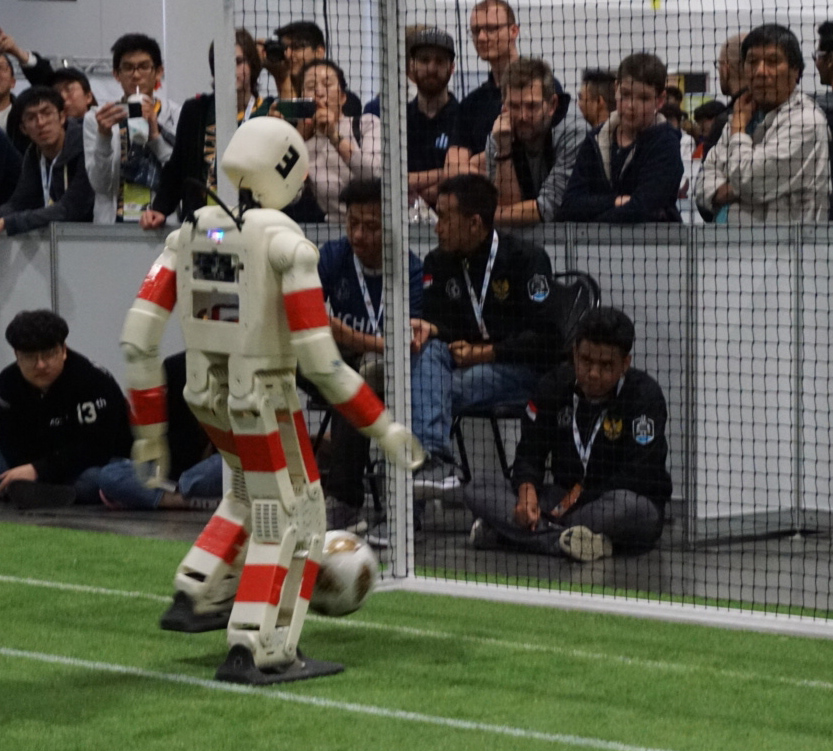
\includegraphics[height=4in]{img/nimbro_robot.jpg}
\captionsetup{labelformat=empty}
\caption{Team NimbRo, winner of the Best Humanoid Award 2018}
\end{figure}

{\large Changes are either \added{marked in magenta text colour} (for additions) or by  \removed{crossed out text} (for deletions).}

\bigskip
RoboCup Humanoid League Mailing List (for important announcements):\\
\url{https://mailman.cc.gatech.edu/mailman/listinfo/robocup-humanoid}

\medskip
RoboCup Humanoid Forum (for rule discussion and questions):\\
\url{https://hl.forum.robocup.org}

\medskip
RoboCup Humanoid League Home Pages:\\
\url{https://www.robocuphumanoid.org/}\\
\url{https://www.robocup.org/leagues/3}

\medskip
Inspired by the \href{https://resources.fifa.com/image/upload/laws-of-the-game-2018-19.pdf?cloudid=khhloe2xoigyna8juxw3}{\textcolor[rgb]{0,0,0.5}{Laws of the Game of the International Football Association Board}},\\
with amendments for the RoboCup Humanoid League.

\setcounter{figure}{0}

\clearpage

{\bfseries\color[rgb]{0.4,0.4,0.4}
Overview}

\bigskip

Section I -- Laws of the Game

\bigskip

Section II -- RoboCup Humanoid League Competition Rules

\bigskip

Section III -- Rules for RoboCup Humanoid League Technical Challenges

\clearpage

{\bfseries\color[rgb]{0.4,0.4,0.4}
Contents}

\addtocontents{toc}{\protect\setcounter{tocdepth}{0}}
\renewcommand\contentsname{}
\vspace*{-1cm}
\tableofcontents
\addtocontents{toc}{\protect\setcounter{tocdepth}{2}}


%%%%%%%%%%%%%%%%%%%%%%%%%%%%%%%%%%%%%%%%%%%
%%%%%%%%%%% SECTION I %%%%%%%%%%%%%%%%%%%%%
%%%%%%%%%%%%%%%%%%%%%%%%%%%%%%%%%%%%%%%%%%%

\clearpage

\begin{center}
\Huge\bfseries{
\vspace*{3cm}
Section I

\vspace*{2cm}

Laws of the Game}
\end{center}
\addcontentsline{toc}{section}{Section I: Laws of the Game}

\vspace*{12cm}

The Laws of the Game should be updated regularly to refer to the most
recent FIFA document.

\bigskip

Deviations from the FIFA rules are marked in the text:

\bigskip
\begin{tabular}{ll}
'replaces': &A RoboCup-specific rule temporarily replaces a FIFA rule. \\
'suspended': &A specific FIFA rule is not yet applied. \\
'new': &A RoboCup-specific rule is temporarily introduced.
\end{tabular}


\clearpage
\sffamily
{\bfseries\color[rgb]{0.4,0.4,0.4}
NOTES ON THE LAWS OF THE GAME }

\bigskip

{\color[rgb]{0.4,0.4,0.4}{Modifications} }

Subject to the agreement of the member association concerned and provided the principles of these Laws are maintained, the Laws may be modified in their application for regional matches.

Any or all of the following modifications are permissible: 

\begin{itemize}
\item size of the field of play
\item size, weight and material of the ball
\item width between the goalposts and height of the crossbar from the ground
\item duration of the periods of play
\item substitutions
\end{itemize}

\bigskip

{\color[rgb]{0.4,0.4,0.4}{Male and Female}}

References in respect of referees, assistant referees and officials have been changed from the original FIFA document to a gender neutral language. The reference to players, since they refer to robots in this context, have been kept in the male gender. However, we strongly encourage the FIFA to officially change their laws of the game to fully gender neutral language in the future in respect to all participants in the game.

\greyed{(replaces: References to the male gender in the Laws of the Game in respect of referees, assistant referees, players and officials are for simplification and apply to both men and women.)}

\bigskip

{\color[rgb]{0.4,0.4,0.4}{Official languages}}

RoboCup Humanoid League Technical Committee publishes the Laws of the Game in English.

\bigskip

{\color[rgb]{0.4,0.4,0.4}{Key} }

A single line in the left-hand margin indicates new Law changes.

\clearpage

\clearpage
\sffamily
{\bfseries\color[rgb]{0.4,0.4,0.4}
Law 1 -- The Field of Play}
\phantomsection
\addcontentsline{toc}{subsection}{Law 1 -- The Field of Play}

\bigskip
{\bfseries Field surface}

\headlinebox
 
Matches may be played on artificial surfaces with a height of approximately 30 mm.

\greyed{
(replaces: Matches may be played on natural or artificial surfaces, according to the rules of the competition.)}


\bigskip

{\sffamily
The colour of artificial surfaces must be green. }




\greyed{\bigskip
(suspended: Where artificial surfaces are used in either competition matches between representative teams of member associations affiliated to FIFA or international club competition matches, the surface must meet the requirements of the FIFA Quality Concept for Football Turf or the International Artificial Turf Standard, unless special dispensation is given by FIFA.) }


\bigskip

{\bfseries
Field markings}

\headlinebox

The field of play must be rectangular and marked with lines. These lines belong to the areas of which they are boundaries.

\bigskip

The two longer boundary lines are called touch lines. The two shorter lines are called goal lines.

\bigskip

The field of play is divided into two halves by a halfway line, which joins the midpoints of the two touch lines.

\bigskip

The centre mark is indicated at the midpoint of the halfway line. A circle with a radius of 0.75 m \added{for KidSize and TeenSize and 1.5 m for AdultSize} is marked around it.
\greyed{(replaces: A circle with a radius of 9.15 m (10 yds) is marked around it.)}



\greyed{\bigskip
(suspended: Marks may be made off the field of play, 9.15 m (10 yds) from the corner arc and at right angles to the goal lines and the touch lines, to ensure that defending players retreat this distance when a corner kick is being taken.) }

\bigskip

{\textbf{Dimensions}}

\headlinebox

The length of the touch line must be greater than the length of the goal line. 

\bigskip

\added{KidSize and TeenSize matches} 

\begin{tabular}{lll}
Length (touch line): &approximately &9 m \\
Width (goal line): &approximately &6 m
\end{tabular}

\greyed{
(replaces:

\begin{tabular}{lll}
Length (touch line): &minimum &90 m \\
&maximum &120 m \\
Width (goal line): &minimum &45 m \\
&maximum &90 m)
\end{tabular}
}

\bigskip

All lines must be of the same width, which must be approximately 5 cm. 

\greyed{
(replaces: All lines must be of the same width, which must be not more than 12 cm (5 ins).)}


\bigskip

\removed{International matches} \added{AdultSize matches}

\begin{tabular}{lll}
Length (touch line): &approximately &\removed{9 m} \added{14 m} \\ 
Width (goal line): &approximately &\removed{6 m} \added{9 m }\\
\end{tabular}

\greyed{
(replaces: 

\begin{tabular}{lll}
Length (touch line): &minimum &100 m \\
&maximum &110 m \\
Width (goal line): &minimum &64 m \\
&maximum &75 m)
\end{tabular}
}

\bigskip

{\bfseries The goal area }

\headlinebox

Two lines are drawn at right angles to the goal line, 1.2 m from the inside of each goalpost. These lines extend into the field of play for a distance of 1 m and are joined by a line drawn parallel with the goal line. The area bounded by these lines and the goal line is the goal area. 

\greyed{
(replaces: Two lines are drawn at right angles to the goal line, 5.5 m (6 yds) from the inside of each goalpost. These lines extend into the field of play for a distance of 5.5 m (6 yds) and are joined by a line drawn parallel with the goal line. The area bounded by these lines and
the goal line is the goal area. )}

\bigskip

{\bfseries The penalty area }

\headlinebox

\greyed{
(suspended: Two lines are drawn at right angles to the goal line, 16.5 m (18 yds) from the inside of each goalpost. These lines extend into the field of play for a distance of 16.5 m (18 yds) and are joined by a line drawn parallel with the goal line. The area bounded by these lines and the goal line is the penalty area.) \bigskip}



A penalty mark is made at 2.1m \added{for AdultSize and 1.5m for KidSize and TeenSize} from the midpoint between the goalposts and equidistant to them. 
\greyed{(replaces: Within each penalty area, a penalty mark is made 11 m (12 yds) from the midpoint between the goalposts and equidistant to them.)\bigskip}



\greyed{
(suspended: An arc of a circle with a radius of 9.15 m (10 yds) from the centre of each penalty mark is drawn outside the penalty area.)}

\simplify{
\bigskip

{\textbf{Flagposts} }

\headlinebox

\greyed{
(suspended: A flagpost, not less than 1.5 m (5 ft) high, with a non-pointed top and a flag must be placed at each corner.) }

\bigskip

\greyed{
(suspended: Flagposts may also be placed at each end of the halfway line, not less than 1 m (1 yd) outside the touch line.)}

\bigskip

{\bfseries The corner arc }

\headlinebox

\greyed{
(suspended: A quarter circle with a radius of 1 m (1 yd) from each corner flagpost is drawn inside the field of play.)}
}

\bigskip

{\bfseries Goals }

\headlinebox

A goal must be placed on the centre of each goal line.


\bigskip

A goal consists of two upright posts equidistant from the corner flagposts and joined at the top by a horizontal crossbar. The goalposts and crossbar must be made of wood, metal or other approved material. They must be square, rectangular, round or elliptical in shape and must
not be dangerous to players.

\bigskip

The distance between the posts is 2.6 m and the distance from the lower edge of the crossbar to the ground is 1.8 m. 

\greyed{
(replaces: The distance between the posts is 7.32 m (8 yds) and the distance from the lower edge of the crossbar to the ground is 2.44 m (8 ft).)}

\bigskip

\greyed{
(suspended: figures of different goal post geometries)}

\bigskip

\greyed{
(suspended: The position of the goalposts in relation to the goal line must be according to the graphics below.)}

\bigskip

If the shape of the goalposts is square (viewed from above), the sides must be parallel or perpendicular to the goal line. The sides of the crossbar must be parallel or perpendicular to the field plane.

\bigskip

If the shape of the goalposts is elliptical (viewed from above), the longest axis must be perpendicular to the goal line. The longest axis of the crossbar must be parallel to the field plane.

\bigskip

If the shape of the goalposts is rectangular (viewed from above), the longest side must be perpendicular to the goal line. The longest side of the crossbar must be parallel to the field plane.

\bigskip

Both goalposts and the crossbar have the same width and depth, which do not exceed 12 cm (5 ins).
The goal lines must be approximately 5 cm of width. 
\greyed{
(replaces: The goal lines must be of the same width as the goalposts and the crossbar.)} 
Nets (new:) which must not be green or white may be attached to the goals and the ground behind the goal, provided that they are properly supported and do not interfere with the goalkeeper. 

\bigskip

The goalposts and crossbars must be white.

\bigskip

{\bfseries Safety}

\headlinebox

Goals must be anchored securely to the ground. Portable goals may only be used if they satisfy this requirement.

\bigskip

{\bfseries The field of play}

\headlinebox 

\begin{center}
\begin{figure}[h]
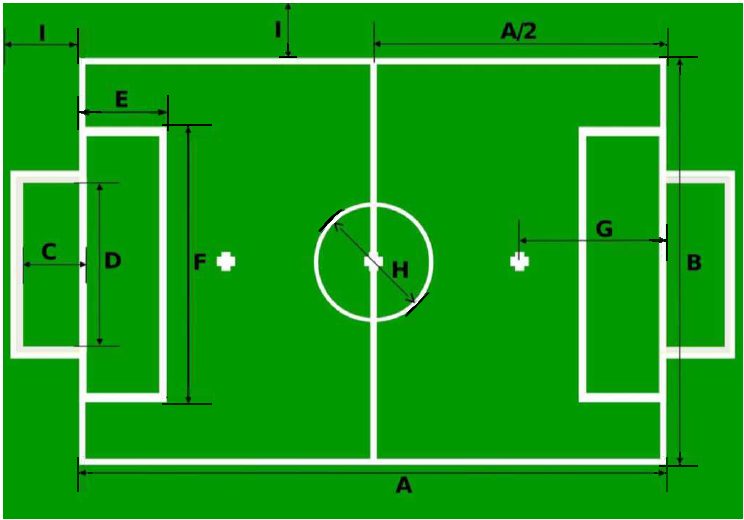
\includegraphics[width=\textwidth]{img/field.png}
\caption{Humanoid robot soccer field (not to scale)}
\end{figure}
\end{center}
\newpage

\begin{center}
\tablehead{}
\begin{table}[h]
\caption{Approximate dimensions of the rectangular field of soccer play.}
\centering
\begin{tabular}{|l|l|c|c|}
\hline
& & KidSize and TeenSize & \added{AdultSize} \\
\hline
A & Field length & 9 m & \added{14 m}\\
\hline
B & Field width &  6 m & \added{9 m}\\
\hline
C & Goal depth & \multicolumn{2}{c|}{0.6 m}\\
\hline
D & Goal width & \multicolumn{2}{c|}{2.6 m}\\
\hline
~ & Goal height & \multicolumn{2}{c|}{1.8 m}\\
\hline
E & Goal area length & \multicolumn{2}{c|}{1 m}\\
\hline
F & Goal area width & \multicolumn{2}{c|}{5 m}\\
\hline
G & Penalty mark distance & \removed{2.1} \added{1.5} m & 2.1 m\\
\hline
H & Centre circle diameter & 1.5 m & \added{3 m}\\
\hline
I & Border strip width (min.) & 0.7 m & \added{1 m}\\
\hline
\end{tabular}
\end{table}
\end{center}

\greyed{
(replaces figure of field)}

\bigskip

\added{{\bfseries Light Condition}}

\headlinebox 

\added{The lighting could either be artificial or natural.}

\simplify{
\bigskip

{\bfseries Corner flagpost}

\headlinebox 

\greyed{(suspended: figure of flagpost)}

\bigskip

{\bfseries Metric measurements}

\headlinebox 

\greyed{(suspended: figure with metric dimensions of field)}

\bigskip

{\bfseries Imperial measurements}

\headlinebox 

\greyed{(suspended: figure with imperial dimensions of field)}
}

\simplify{
\clearpage

{\bfseries Decisions of the International F.A. Board}

\headlinebox 

\greyed{
(suspended: Decision 1

Where a technical area exists, it must meet the requirements approved by the International F.A. Board, which are contained in the section of this publication entitled The Technical Area.)}

\bigskip

\greyed{
(suspended: Decision 2

Where goal-line technology (GLT) is used, modifications to the goal frame may be allowed. They must be in accordance with the specifications stipulated in the FIFA Quality Programme for GLT and according to the above description, ``Goals''.) }
}

\clearpage
\sffamily
{\bfseries\color[rgb]{0.4,0.4,0.4}
Law 2 -- The Ball}
\addcontentsline{toc}{section}{LAW 2 -- The Ball}


\bigskip

{\bfseries Qualities and measurements }

\headlinebox

The ball is:

\begin{itemize}
\item spherical
\item made of leather or other suitable material
\item FIFA size 1 for KidSize, size 3 for TeenSize and size 5 for AdultSize leagues. 
\textcolor[rgb]{0.4,0.4,0.4}{(replaces: of a circumference of not more than 70 cm (28 ins) and not less than 68 cm (27 ins) and: not more than 450 g (16 oz) and not less than 410 g (14 oz) in weight at the start of the match)}
\item {\color[rgb]{0.4,0.4,0.4}
(suspended: of a pressure equal to 0.6 -- 1.1 atmosphere (600 -- 1,100 g/cm2) at sea level (8.5 lbs/sq in -- 15.6 lbs/sq in)) }
\end{itemize}

\bigskip

{\bfseries Replacement of a defective ball }

\headlinebox

If the ball bursts or becomes defective during the course of a match:

\begin{itemize}
\item the match is stopped
\item the match is restarted by dropping the replacement ball at the place where the original ball became defective, unless play was stopped inside the goal area, in which case the referee drops the replacement ball on the goal area line parallel to the goal line at the point
nearest to where the original ball was located when play was stopped
\end{itemize}

If the ball bursts or becomes defective during a penalty kick or during kicks from the penalty mark as it moves forward and before it touches any player or the crossbar or goalposts: 

\begin{itemize}
\item the penalty kick is retaken
\end{itemize}

If the ball bursts or becomes defective whilst not in play at a kick-off, goal kick, corner kick, free kick, penalty kick or throw-in:

\begin{itemize}
\item the match is restarted accordingly
\end{itemize}

The ball may not be changed during the match without the authority of the referee.

\clearpage

{\bfseries Decisions of the International F.A. Board}

\headlinebox

Decision 1

{\color[rgb]{0.4,0.4,0.4}
(suspended: In addition to the requirements of Law 2, acceptance of a ball for use in matches played in an official competition organised under the auspices of FIFA or the confederations is conditional upon the ball bearing one of the following: 

\begin{itemize}
\item the official ``FIFA APPROVED'' logo 
\item the official ``FIFA INSPECTED'' logo
\item the ``INTERNATIONAL MATCHBALL STANDARD'' logo
\end{itemize}

Such a logo on a ball indicates that it has been tested officially and found to be in compliance with specific technical requirements, different for each logo and additional to the minimum specifications stipulated in Law 2. The list of the additional requirements specific
to each of the respective logos must be approved by the International F.A. Board. The institutes conducting the tests are subject to the approval of FIFA.

\bigskip

Member association competitions may also require the use of balls bearing any one of these three logos.

\bigskip

(figures...))}

\bigskip

Decision 2

{\color[rgb]{0.4,0.4,0.4}
(suspended: In matches played in an official competition organised under the auspices of FIFA, the confederations or the member associations, no form of commercial advertising on the ball is permitted, except for the
emblem of the competition, the competition organiser and the authorised trademark of the manufacturer. The competition regulations may restrict the size and number of such markings.)}

\bigskip

Decision 3

{\sffamily\color[rgb]{0.4,0.4,0.4}
(suspended: Where goal-line technology (GLT) is used, balls with integrated technology are allowed, but they must either be ``FIFA APPROVED'', ``FIFA INSPECTED'' or 
``INTERNATIONAL MATCHBALL STANDARD'' (see ``Decision 1'').) }
\clearpage
\sffamily

{\bfseries\color[rgb]{0.4,0.4,0.4}
Law 3 -- The Players}
\phantomsection
\addcontentsline{toc}{subsection}{Law 3 -- The Players}


\bigskip

{\bfseries Number of Players}

\headlinebox

A match is played by two teams, each consisting of not more than four players in KidSize
\removed{, not more than three players in TeenSize} and not more than two players in AdultSize,
one of whom must be designated as goalkeeper.
A match may not start if either team consists of less than one player.
If a team has not at least one player (who may be incapable to play) at the side of the field,
it is considered a forfeit.

\greyed{
(replaces: A match is played by two teams, each consisting of not more than eleven players, one of whom is the goalkeeper. A match may not start if either team consists of fewer than seven players.)}

\bigskip

{\bfseries Number of substitutions}

\headlinebox
 
{\bfseries Official competitions }

Up to a maximum of two \greyed{(replaces: three)} substitutes may be used in any match played in an official competition organised under the auspices of FIFA, the confederations or the member associations.

The rules of the competition must state how many substitutes may be nominated, from two \greyed{(replaces: three)} up to a maximum of twelve.

\bigskip

\greyed{
(suspended:
\simplify{
{\bfseries Other matches }

In national ``A'' team matches, up to a maximum of six substitutes may be used.

\bigskip

In all other matches, a greater number of substitutes may be used provided that:

\begin{itemize}
\item the teams concerned reach agreement on a maximum number 
\item the referee is informed before the match
\end{itemize}

If the referee is not informed, or if no agreement is reached before the match, no more than six substitutes are allowed.}

\bigskip
}

{\bfseries Substitution procedure}

\headlinebox

In all matches, the names of the substitutes must be given to the referee prior to the start of the match. Any substitute whose name is not given to the referee at this time may not take part in the match.

\bigskip

To replace a player with a substitute, the following conditions must be observed:

\begin{itemize}
\item the referee must be informed before any proposed substitution is made
\item the substitute only enters the field of play after the player being replaced has left and after receiving a signal from the referee
\item the substitute only enters the field of play at the penalty mark of the player's own half \greyed{
(replaces: the halfway line)} and during a stoppage in the match 
\item the substitution is completed when a substitute enters the field of play
\item from that moment, the substitute becomes a player and the player he has replaced becomes a substituted player 
\item \greyed{(suspended: the substituted player takes no further part in the match)}
\item all substitutes are subject to the authority and jurisdiction of the referee, whether called upon to play or not
\end{itemize}

{\bfseries Changing the goalkeeper}

\headlinebox

Any of the other players may change places with the goalkeeper, provided that:

\begin{itemize}
\item the referee is informed before the change is made
\item the change is made during a stoppage in the match
\end{itemize}

{\bfseries Infringements and sanctions}

\headlinebox

If a substitute or substituted player or a team official enters the field of play
without the referee's permission:

\begin{itemize}
\item the referee stops play (although not immediately if the substitute or substituted player does not interfere with play)
\item the referee cautions him for unsporting behaviour and orders him to leave the field of play 
\item if the referee has stopped play, it is restarted with an direct free kick
      for the opposing team from the position of the ball at the time of the
      stoppage (see Law 13 -- Position of free kick)
\end{itemize}

\bigskip

If a named substitute enters the field of play instead of a named player at the start of the match and the referee is not informed of this change:

\begin{itemize}
\item the referee allows the named substitute to continue the match 
\item no disciplinary sanction is taken against the named substitute 
\item the number of substitutions allowed by the offending team is not reduced 
\item the referee reports the incident to the appropriate authorities
\end{itemize}

\bigskip

If a player changes places with the goalkeeper without the
referee's permission before the change is made: 

\begin{itemize}
\item the referee allows play to continue
\item the referee cautions the players concerned when the ball is next out of play
\end{itemize}

\bigskip

In the event of any other infringements of this Law:

\begin{itemize}
\item the players concerned are cautioned
\item the match is restarted with an indirect free kick, to be taken by a player of the opposing team from the position of the ball at the time of the stoppage (see Law 13 -- Position of free kick)
\end{itemize}

\bigskip

{\bfseries Players and substitutes sent off}

\headlinebox

A player who has been sent off before the kick-off may be replaced only by one of the named substitutes.

\bigskip

A named substitute who has been sent off, either before the kick-off or after play has started, may not be replaced.

\clearpage
\sffamily
{\bfseries\color[rgb]{0.4,0.4,0.4}
Law 4 -- The Players ('Equipment')}
\phantomsection
\addcontentsline{toc}{subsection}{Law 4 -- The Players ('Equipment')}

\bigskip

{\bfseries Safety }

\headlinebox

A player must not use equipment or wear anything that is dangerous to himself or another player (including any kind of jewellery).

\bigskip

{\bfseries The Design of the Robots (new)}

\headlinebox

Robots participating in the Humanoid League competitions must have a human-like body plan, as shown in Fig. \ref{fig:bodyplan}. They must consist of two legs, two arms, and one head, which are attached to a trunk.

\bigskip

(new:) Robots in \added{KidSize} \removed{kid and teen size sub-leagues} must be
equipped with a handle, to be picked up safely and with no harm to the robot and
the handler.


\begin{figure}[h]
\begin{center}
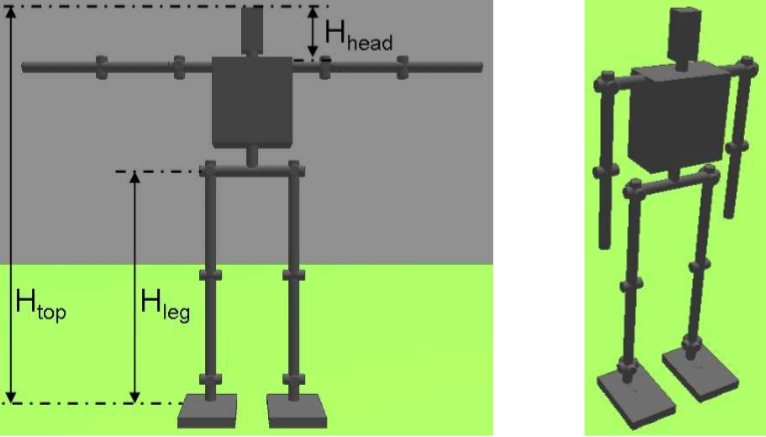
\includegraphics[width=0.7\textwidth]{img/bodyplan.png}
\caption{Example of a humanoid robot body plan (left) and standing upright pose (right)}
\label{fig:bodyplan}
\vspace{-3ex}
\end{center}
\end{figure}


The robots must be able to stand upright on their feet and to walk on their legs.
KidSize \removed{and TeenSize} robots need to be able to recover from a fall
(get back to a standing position).
The only allowed modes of locomotion are bipedal walking, running and jumping.

\bigskip

All actions of the robots must be kinematically equivalent to humanoid motions.

\bigskip

\added{Robots must be equipped with an emergency stop button that makes the robot immediately desist with all motions, or ideally go limp and/or cut power to the actuators. In addition to the emergency stop button, robots may only have up to two additional physical or virtual buttons: One to start the robot behaviour and one to stop the behaviour. The buttons must be clearly labelled. If the robot has more buttons that cannot be detached, they must be visibly masked during the games.}

\bigskip

{\bfseries Robot Height (new)}

\headlinebox

Based on $H_{top}$, the following size restrictions apply:

\begin{itemize}
\item 40 cm ${\leq}$ $H_{top}$ ${\leq}$ \removed{90} \added{100} cm to play in the KidSize class,
\item \removed{80 cm ${\leq}$ $H_{top}$ ${\leq}$ 140 cm to play in the TeenSize class,}
\item \removed{130} \added{100} cm ${\leq}$ $H_{top}$ ${\leq}$
      \removed{180} \added{200} cm to play in the AdultSize class.
\end{itemize}

$H_{top}$ is defined as the height of the robot when standing upright (with fully extended knees, cf. Fig. \ref{fig:bodyplan} right) and $H_{COM}$ denotes the height of the robot's centre of mass, measured in upright posture. $H_{top}$ is measured with the head of the robot oriented in such a way that it is tilted to either its maximum upwards tilt angle or the horizon line, whichever is lower.

\bigskip

{\bfseries Weight Restrictions (new)}

\headlinebox

\begin{itemize}
\item \removed{The maximum weight for robots allowed to play in the TeenSize class is 20 kg.}
\item \removed{The minimum weight for robots allowed to play in the AdultSize class is 10 kg.}
\end{itemize}

\added{
The robot BMI, Body-Mass Index, is defined as following:
$\mathrm{BMI} = \frac{M}{{H_{top}}^2}$,
where $M$ is the mass of the robot in kg and $H_{top}$ its height in meters.
The following restriction applies:
}
\begin{itemize}
\item \added{$5 \leq \mathrm{BMI} \leq 30$}
\end{itemize}

\bigskip

{\bfseries Size Restrictions (new)}

\headlinebox

All robots participating in the Humanoid League must comply with the following restrictions:

\begin{itemize}
\item Each foot must fit into a rectangle of area $\tfrac{1}{32} (2.2 \cdot H_{COM})^2$.
      A foot is defined as the minimum encapsulating rectangle covering all
      mechanical parts below the ankle joint.
      The encapsulating rectangle should be in a plane parallel to the bottom
      contact surface of the foot.
\item The ratio between the longest and the shortest side of the encapsulating
      rectangle should be between $1.2$ and $3.5$
\item The robot must fit into a cylinder of diameter $0.55 \cdot H_{top}$.
\item The robot does not possess a configuration where it is extended longer than 1.5{\textperiodcentered}$H_{top}$ .
\item The length of the legs $H_{leg}$, including the feet, satisfies 0.35{\textperiodcentered}$H_{top}$ ${\leq}$ $H_{leg}$ ${\leq}$ 0.7{\textperiodcentered}$H_{top}$ .
\item The height of the head $H_{head}$, including the neck,
  satisfies \added{$0.1 \cdot H_{top} \leq H_{head} \leq 0.3 \cdot H_{top}$}\\
  \removed{$0.05 \cdot H_{top} \leq H_{head} \leq 0.25 \cdot H_{top}$}.
  $H_{head}$ is defined as the vertical distance from the axis of the first arm
  joint at the shoulder to the top of the head.
\item The leg length is measured while the robot is standing up straight. The length is measured from the first rotating joint where its axis lies in the plane parallel to the standing ground to the tip of the foot.
\item The minimum length of the arm, measured from the first joint, is $H_{top} - H_{leg} - H_{head}$.
\end{itemize}


{\bfseries Sensors (new)}

\headlinebox

Teams participating in the Humanoid League competitions are encouraged to equip their robots with sensors that have an equivalent in human senses. These sensors must be placed at a position roughly equivalent to the location of the human{\textquoteright}s biological sensors. In particular, 

\begin{itemize}
\item The only active external sensor allowed is sound
(``human-like'' with respect to volume and frequency) with one loudspeaker on the robot. The loudspeaker may be placed in the head, neck or trunk of the robot. Any
other active sensor (emitting light, sound, or electromagnetic waves into the environment in order to measure reflections) is not allowed. 
\item External sensors, such as cameras and up to two microphones, may not be placed in the legs or arms or the
torso of the robots. They must be placed in the robot's
head and above any neck joint. 
\item The number of cameras is limited to a stereo vision setup (i.e., max. 2 cameras with a large overlap) only. Monocular vision is also allowed.
\item The field of view of the robots is limited at any time to $180$ degrees. This means that the maximum angle between any two points in the union of the field of view of all cameras mounted on the robot must be less than $180$ degrees. Also the pan-tilt motion of the head and the cameras mounted on the robot's head is restricted to be more human like not only with respect to the field of view but also to the range of motion of the neck joints. Therefore, the mechanism to pan the camera is limited to $270$ degree pan, which means $\pm135$ degrees from the position looking straight ahead. The mechanism to tilt the camera is limited to $\pm90$ degrees (measured from the horizontal line). Furthermore, if positioned at the centre mark the robot may not be able to see more than two goal posts in any tilt angle and in any standing or walking posture of the robot. 
\item Touch sensors, force sensors, and temperature sensors may be placed at any position on the robot.
\item Sensors inside the robot may measure all quantities representing the local state of the system, including (but not limited to) voltages, currents, forces, movements, accelerations, and rotational speeds. They can be at any position inside the robot. Measurements from earth magnetic field sensors may not be used in the software and - in case of doubt - the code must be made available to members of the Technical Committee for inspection.
\end{itemize}

{\bfseries Communication and Control (new)}

\headlinebox

Robots participating in the Humanoid League competitions must act autonomously while a competition is running. No external power supply, teleoperation, remote control, or remote brain of any kind is allowed.

\bigskip

Robots may communicate only via the wireless network provided by the organizers, which must support the referee box. The total bandwidth of the robots belonging to one team may not exceed 1 Mbit/s. The robots must not rely on the quality of the wireless network. They
must be able to play if the network is of low quality. Only robots are allowed to communicate by WLAN. Any other computers of team members are only allowed to communicate by tethered LAN. No other wireless communication is allowed onsite. All other wireless hardware must be deactivated. A team may be disqualified if one of the team members violates this rule.

\bigskip

Robots in play may communicate with each other at any time during a game.
Robots not currently in play may only send status updates about their own
internal hardware or software functionality over the network.
They may not communicate any game relevant information.
Any kind of transmission from an external computer or an out of play robot to
the playing robots is prohibited.
This implies that any monitoring is only done by receiving UDP communication
from the robots using an external computer connected by tethered LAN to the
official wireless router. 

\bigskip

Sending any direct or indirect transmission from an external computer to the
robots has to take place during a timeout or any form of temporal absence and
outside the field of play.
Any time the robot handler or another team member is touching the robot,
a cable is connected or another form of communication with the robot
(including button clicks) take place, the robot is considered in service.
The regular penalty time will start counting only after any type of
communication with the robot has finished and will be reset whenever the robot
handler attempts to service the robot again.

\bigskip


Teams may not use any type of communication, excluding verbal communication,
with robots in play, in service or with robots serving their 30 seconds penalty
time that contains information which reduces the need for autonomy in detecting
the current game state of the robots, including the position of the ball,
the location where the robot re-enters the field,
the orientation of the robots own or opponents goal,
and the position of team members or opponents.
In case of doubt that a team violates this rule,
the code must be made available to members of the Technical Committee for inspection.

\bigskip

During the game an official game controller/referee box will be used.
It uses UDP to broadcast information to the robots like elapsed time,
current score, game state (ready, set, playing, finished) and the robot-specific
penalized state. The source code is open.
\added{Teams have to be able to use the referee box in order to respect the rules.}
\removed{To encourage teams to use the referee box, 15 seconds advantage is
given to teams using the referee box in any stoppage of the game.}



\bigskip

In KidSize \removed{and TeenSize}, no humans are allowed on the field while the
ball is in play.
Robot handlers stay in a designated area and must receive permission from the
referee prior to entering the field.
Each team may designate only one person as robot handler.
The robot handler of a team may not touch a robot of another team in order to
avoid any (unintentional or intentional) damage to that robot. 

\bigskip

The source code of the game controller/referee box is available from

\textcolor[rgb]{0.0,0.0,0.49803922}{https://github.com/RoboCup-Humanoid-TC/GameController},
see also 

\textcolor[rgb]{0.0,0.0,0.49803922}{https://www.robocuphumanoid.org}.

\simplify{
\bigskip

\newpage
\greyed{
{\bfseries (suspended: Basic equipment}

\headlinebox

The basic compulsory equipment of a player comprises the following separate items:

\begin{itemize}
\item a jersey or shirt with sleeves -- if undergarments are worn, the colour of the sleeve must be the same main colour as the sleeve of the jersey or shirt 
\item shorts -- if undershorts or tights are worn, they must be of the same main colour as the shorts
\item stockings -- if tape or similar material is applied externally it must be the same colour as that part of the stocking it is applied to shinguards footwear) 
\end{itemize}
}

\bigskip

\greyed{
{\bfseries (suspended: Shinguards}

\headlinebox

\begin{itemize}
\item are covered entirely by the stockings
\item are made of rubber, plastic or a similar suitable material 
\item provide a reasonable degree of protection)
\end{itemize}
}
}

\bigskip

{\bfseries Colours}

\headlinebox

\begin{itemize}
\item (new) Robots must be mostly black or of dark grey colour (i.e. RAL 7011 Iron Grey or darker) and non reflective. Robots may also be coloured in aluminimum-like silver, grey or white but then their feet must be coloured black. Any colour used for the field (green, white) or colours similar to the opponent team's team markers must be avoided. Arms, legs and bodies of the robot must be of solid shape appearance.
\item (new) The robots must be marked with team markers.
      These markers are coloured red for one team and blue for the other team.
      The total visible area of all team markers (up to 20) on the robot's arms,
      legs and chest combined must be at least $0.06\cdot {H_{top}}^2$.
      The visible area of the one to five largest team markers on each side
      (left, right, front and back) must be at least $0.015\cdot {H_{top}}^2$.
      If both teams cannot agree, which team colour to use, a coin will be
      flipped an hour prior to the game to assign the team colours.
\item (new) The robots of each team must be uniquely identifiable. They must be marked with numbers or names. The goal keeper robot must be marked uniquely that it can be easily distinguished from the other robots of a team by the referees. 
\item The two teams must wear colours that distinguish them from each other and also the referee and the assistant referees.
\greyed{\item 
(suspended: Each goalkeeper must wear colours that distinguish him from the other players, the referee and the assistant referees) }
\end{itemize}

\bigskip

{\bfseries Infringements and sanctions}

\headlinebox

In the event of any infringement of this Law:

\begin{itemize}
\item play need not be stopped
\item the player at fault is instructed by the referee to leave the field of play to correct his equipment
\item the player leaves the field of play when the ball next ceases to be in play, unless he has already corrected his equipment
\item any player required to leave the field of play to correct his equipment must not re-enter without the referee's permission
\item the referee checks that the player's equipment is correct before allowing him to re-enter the field of play 
\item the player is only allowed to re-enter the field of play before the respective penalty time is over \greyed{ (replaces: when the ball is out of play)}
\end{itemize}

\bigskip

A player who has been required to leave the field of play because of an infringement of this Law and who re-enters the field of play without the referee's permission must be cautioned.

\bigskip

\clearpage
{\bfseries Restart of play}

\headlinebox

If play is stopped by the referee to administer a caution:

\begin{itemize}
\item the match is restarted by an indirect free kick taken by a player of the opposing team from the place where the ball was located when the referee stopped the match (see Law 13 -- Position of free kick)
\end{itemize}

\bigskip


{\bfseries Decisions of the International F.A. Board }

\headlinebox

Decision 1

Players must not reveal undergarments showing slogans or advertising. The basic compulsory equipment must not have any political, religious or personal statements. A player removing his jersey or shirt to reveal slogans or advertising will be sanctioned by the competition organiser. The team of a player whose basic compulsory equipment has political, religious or personal slogans or statements will be sanctioned by the competition organiser (new) or by RoboCup Federation Humanoid League.

\clearpage
\sffamily
{\bfseries\color[rgb]{0.4,0.4,0.4}
Law 5 -- The Referee}
\phantomsection
\addcontentsline{toc}{subsection}{Law 5 -- The Referee}

\bigskip

{\bfseries The authority of the referee}

\headlinebox

Each match is controlled by a referee who has full authority to enforce the Laws of the Game in connection with the match to which they have been appointed. \added{Decisions will be made to the best of the referees ability according to the Laws of the Game and the spirit of the game and will be based on the opinion of the referee who has the discretion to take appropriate action within the framework of the Laws of the Game.}

\bigskip

{\bfseries Powers and duties}

\headlinebox

The Referee:

\begin{itemize}
\item enforces the Laws of the Game
\item controls the match in cooperation with the assistant referees and, where applicable, with the fourth official
\item ensures that any ball used meets the requirements of Law 2 
\item ensures that the players' equipment meets the requirements of Law 4
\item acts as timekeeper and keeps a record of the match
\item stops, suspends or abandons the match, at their discretion, for any infringements of the Laws
\item stops, suspends or abandons the match because of outside interference of any kind
\item stops the match if, in their opinion, a player is seriously injured and ensures that he is removed from the field of play. An injured player may only return to the field of play after the respective penalty time is over \greyed{ (replaces: after the match has restarted)}
\item allows play to continue until the ball is out of play if a player is, in their opinion, only slightly injured 
\item ensures that any player bleeding from a wound leaves the field of play. The player may only return on receiving a signal from the referee, who must be satisfied that the bleeding has stopped
\item allows play to continue when the team against which an offence has been committed will benefit from such an advantage and penalises the original offence if the anticipated advantage does not ensue at that time
\item punishes the more serious offence when a player commits more than one offence at the same time
\item takes disciplinary action against players guilty of cautionable and sending-off offences. They are not obliged to take this action immediately but must do so when the ball next goes out of play 
\item takes action against team officials who fail to conduct themselves in a responsible manner and may, at their discretion, expel them from the field of play and its immediate surrounds 
\item acts on the advice of the assistant referees regarding incidents that they has not seen 
\item ensures that no unauthorised persons enter the field of play 
\item indicates the restart of the match after it has been stopped 
\item provides the appropriate authorities with a match report, which includes information on any disciplinary action taken against players and/or team officials and any other incidents that occurred before, during or after
the match 
\end{itemize}

\bigskip

{\bfseries Decisions of the referee}

\headlinebox

The decisions of the referee regarding facts connected with play, including whether or not a goal is scored and the result of the match, are final.

\bigskip

The referee may only change a decision on realising that it is incorrect or, at their discretion, on the advice of an assistant referee or the fourth official, provided that they have not restarted play or terminated the match.


\clearpage
{\bfseries Decisions of the International F.A. Board }

\headlinebox

Decision 1

A referee (or where applicable, an assistant referee or fourth official) is not held liable for:

any kind of injury suffered by a player, official or spectator

any damage to property of any kind

any other loss suffered by any individual, club, company, association or other body, which is due or which may be due to any decision that they may take under the terms of the Laws of the Game or in respect of the normal procedures required to hold, play and control a match.

\bigskip

Such decisions may include:

\begin{itemize}
\item a decision that the condition of the field of play or its surrounds or that the weather conditions are such as to allow or not to allow a match to take place
\item a decision to abandon a match for whatever reason
\item a decision as to the suitability of the field equipment and ball used during a match
\item a decision to stop or not to stop a match due to spectator interference or any problem in spectator areas 
\item a decision to stop or not to stop play to allow an injured player to be removed from the field of play for treatment 
\item a decision to require an injured player to be removed from the field of play for treatment 
\item a decision to allow or not to allow a player to wear certain apparel or equipment 
\item a decision (where they have the authority) to allow or not to allow any persons (including team or stadium officials, security officers, photographers or other media representatives) to be present in the vicinity of the field of play 
\item any other decision that they may take in accordance with the Laws of the Game or in conformity with their duties under the terms of FIFA, confederation, member association or league rules or regulations under which the match is played 
\end{itemize}

\bigskip

Decision 2

In tournaments or competitions where a fourth official is appointed, their role and duties must be in accordance with the guidelines approved by the International F.A. Board, which are contained in this publication.

\bigskip

Decision 3

Where goal-line technology (GLT) is used (subject to the respective competition rules), the referee has the duty to test the technology's functionality before the match. The tests to be performed are set out in the FIFA Quality Programme for GLT Testing Manual. If the technology does not function in accordance with the Testing Manual, the referee must not use the GLT system and must report this incident to the respective authority. 

\clearpage
\sffamily
{\bfseries\color[rgb]{0.4,0.4,0.4}
Law 6 -- The Assistant Referees}
\addcontentsline{toc}{section}{LAW 6 -- The Assistant Referees}


\bigskip

{\bfseries Duties}

\headlinebox

Two assistant referees may be appointed whose duties, subject to the decision of the referee, are to indicate:

\begin{itemize}
\item when the whole of the ball leaves the field of play
\item which team is entitled to a corner kick, goal kick or throw-in
\item when a player may be penalised for being in an offside position 
\item when a substitution is requested
\item when misconduct or any other incident occurs out of the view of the referee 
\item when offences have been committed whenever the assistant referees have a better view than the referee (this includes, in certain circumstances, offences committed in the penalty area) 
\item whether, at penalty kicks, the goalkeeper moves off the goal line before the ball is kicked and if the ball crosses the line
\item (new) operate the game controller
\end{itemize}

{\bfseries Assistance}

\headlinebox

The assistant referees also assist the referee in controlling the match in accordance with the Laws of the Game. In particular, they may enter the field of play to help control the distances as defined by the laws of the game 
\textcolor[rgb]{0.4,0.4,0.4}{(replaces: 9.15 m (10 yds)
distance)}.

\bigskip

In the event of undue interference or improper conduct, the referee will relieve an assistant referee of his duties and make a report to the appropriate authorities.
\clearpage
\sffamily
{\bfseries\color[rgb]{0.4,0.4,0.4}
Law 7 -- The Duration of the Match}
\phantomsection
\addcontentsline{toc}{section}{Law 7 -- The Duration of the Match}

\bigskip

{\bfseries Periods of play }

\headlinebox

The match lasts two equal periods of 10 minutes, unless otherwise mutually agreed between the referee and the two teams. Any agreement to alter the duration of the periods of play (e.g. to reduce each half to 8 minutes because of insufficient light) must be made before the start of play and must comply with competition rules.
\greyed{(replaces: The match lasts two equal periods of 45 minutes, unless otherwise mutually agreed between the referee and the two teams. Any agreement to alter the duration of the periods of play (e.g. to reduce each half to 40 minutes because of
insufficient light) must be made before the start of play and must comply with competition rules.)}

\bigskip

{\bfseries Half-time interval}

\headlinebox

Players are entitled to an interval at half-time.

The half-time interval must not exceed 5 minutes.
\greyed{(replaces: The half-time interval must not exceed 15 minutes.) }

Competition rules must state the duration of the half-time interval.

The duration of the half-time interval may be altered only with the consent of the referee. 

\bigskip

{\bfseries Allowance for time lost}

\headlinebox

Allowance is made in either period for all time lost through: 

\begin{itemize}
\item substitutions
\item assessment of injury to players
\item removal of injured players from the field of play for treatment 
\item wasting time
\item any other cause
\end{itemize}

The allowance for time lost is at the discretion of the referee.

\bigskip

{\bfseries Penalty kick}

\headlinebox

If a penalty kick has to be taken or retaken, the duration of either half is extended until the penalty kick is completed.

\bigskip

{\sffamily
\textbf{Abandoned match} }

\headlinebox

An abandoned match is replayed unless the competition rules provide otherwise.
\clearpage
\sffamily
{\bfseries\color[rgb]{0.4,0.4,0.4}
LAW 8 -- The Start and Restart of Play}
\addcontentsline{toc}{section}{LAW 8 -- The Start and Restart of Play}

\bigskip

{\bfseries Definition of kick-off}

\headlinebox

A kick-off is a way of starting or restarting play:

\begin{itemize}
\item at the start of the match 
\item after a goal has been scored 
\item at the start of the second half of the match 
\item at the start of each period of extra time, where applicable
\end{itemize}

A goal may (new:) not be scored directly from the kick-off. (new:) Either the ball must move 20 cm from the kick-off point or must be touched by another player before being kicked into the goal. If the ball is kicked directly into the goal the kick-off is awarded to the opposing team. 

\bigskip

{\bfseries Procedure }

\headlinebox

Before a kick-off at the start of the match or extra time 

\begin{itemize}
\item a coin is tossed and the team that wins the toss decides which goal it will attack in the first half of the match.
\item the other team takes the kick-off to start the match. 
\item the team that wins the toss takes the kick-off to start the second half of the match.
\item in the second half of the match, the teams change ends and attack the opposite goals. 
\end{itemize}

\bigskip

{\bfseries Kick-off}

\begin{itemize}
\item after a team scores a goal, the kick-off is taken by the other team. 
\item all players must be in their own half of the field of play 
\item the opponents of the team taking the kick-off are at least 1.5 m from the ball until it is in play \textcolor[rgb]{0.4,0.4,0.4}{(replaces:
the opponents of the team taking the kick-off are at least 9.15 m (10 yds) from the ball until it is in play)}
\item the ball must be stationary on the center mark
\item the referee gives a signal
\item the ball is in play when it is kicked and moves forward (new: or 10 seconds after the referee gave the signal)
\item {\color[rgb]{0.4,0.4,0.4}
(suspended) the kicker must not touch the ball again until it has touched another player }
\end{itemize}

{\bfseries Infringements and sanctions}

\headlinebox

{\color[rgb]{0.4,0.4,0.4}(suspended: If the player taking the kick-off touches the ball again before it has touched another player:

\begin{itemize}
\item an indirect free kick is awarded to the opposing team to be taken from the position of the ball when the infringement occurred (see Law 13 -- Position of free kick)
\end{itemize}
}

In the event of any other infringement of the kick-off procedure: 

\begin{itemize}
\item the kick-off is retaken
\end{itemize}


{\bfseries Definition of dropped ball}

\headlinebox

A dropped ball is a method of restarting play when, while the ball is still in play, the referee is required to stop play temporarily for any reason not mentioned elsewhere in the Laws of the Game. 

\bigskip

{\bfseries Procedure}

\headlinebox

The game is continued at the center mark. A goal can be scored directly from a dropped ball. The procedure for dropped ball is the same as for kick-off, except that the players of both teams must be outside the center circle. The ball is in play immediately
after the referee gives the signal. If a player moves too close to the ball before the referee gives the signal, a kick-off
is awarded to the opponent team.


{\color[rgb]{0.4,0.4,0.4}{(replaces:
The referee drops the ball at the place where it was located when play was stopped, unless play was stopped inside the goal area, in which case the referee drops the ball on the goal area line parallel to the goal line at the point nearest to where the ball was located when play was stopped.


\bigskip

Play restarts when the ball touches the ground.)}
\color{black}

\bigskip

{\bfseries Infringements and sanctions}

\headlinebox

The ball is dropped again:

\begin{itemize}
\item if it is touched by a player before it makes contact with the ground 
\item if the ball leaves the field of play after it makes contact with the ground, without a player touching it
\end{itemize}

\bigskip

{\color[rgb]{0.4,0.4,0.4}{(suspended:
If the ball enters the goal: 

\begin{itemize}
\item if a dropped ball is kicked directly into the opponents' goal, a goal kick is awarded 
\item if a dropped ball is kicked directly into the team's own goal, a corner kick is awarded to the opposing team
\end{itemize}
}
\clearpage
\sffamily
{\bfseries\color[rgb]{0.4,0.4,0.4}
Law 9 -- The Ball In and Out of Play}
\phantomsection
\addcontentsline{toc}{section}{Law 9 -- The Ball In and Out of Play}

\bigskip

{\bfseries Ball out of play}

\headlinebox

The ball is out of play when:

\begin{itemize}
\item it has wholly crossed the goal line or touch line whether on the ground or in the air
\item play has been stopped by the referee
\end{itemize}

{\bfseries Ball in play }

\headlinebox

The ball is in play at all other times, including when:

\begin{itemize}
\item it rebounds off a goalpost, crossbar or corner flagpost and remains in the field of play
\item it rebounds off either the referee or an assistant referee when they are on the field of play
\end{itemize}
\clearpage
\sffamily
{\bfseries\color[rgb]{0.4,0.4,0.4}{Law 10 -- The Method of Scoring} }
\phantomsection
\addcontentsline{toc}{section}{Law 10 -- The Method of Scoring}

\bigskip

{\bfseries Goal scored }

\headlinebox

A goal is scored when the whole of the ball passes over the goal line, between the goalposts and under the crossbar, provided that no infringement of the Laws of the Game has been committed previously by the team scoring the goal. A goal can only be scored from the respective half of the field.

\bigskip

{\bfseries Winning team}

\headlinebox

The team scoring the greater number of goals during a match is the winner. If both teams score an equal number of goals, or if no goals are scored, the match is drawn. 

\bigskip

{\bfseries Competition rules }

\headlinebox

When competition rules require there to be a winning team after a match or home-and-away tie, the only permitted procedures for determining the winning team are those approved by the International F.A. Board, namely:

\begin{itemize}
\item away goals rule
\item extra time
\item kicks from the penalty mark
\item (new) extended kicks from the penalty mark
\end{itemize}


{\bfseries Goal-line technology (GLT) }

\headlinebox

GLT systems may be used for the purpose of verifying whether a goal has been scored to support the referee{\textquoteright}s decision. The use of GLT must be stipulated in the respective competition rules.
\simplify{\clearpage
\sffamily
{\bfseries\color[rgb]{0.4,0.4,0.4}
(suspended: Law 11 -- Offside)}
\phantomsection
\addcontentsline{toc}{subsection}{Law 11 -- Offside (suspended)}

\bigskip

\greyed{\textbf{Offside position}

\headlinebox

It is not an offence in itself to be in an offside position. A player is in an offside position if:

\begin{itemize}
\item he is nearer to his opponents{\textquoteright} goal line than both the ball and the second-last opponent
\end{itemize}

\bigskip

A player is not in an offside position if:

\begin{itemize}
\item he is in his own half of the field of play or
\item he is level with the second-last opponent or
\item he is level with the last two opponents
\end{itemize}
}

\greyed{\textbf{Offence}

\headlinebox

A player in an offside position is only penalised if, at the moment the ball touches or is played by one of his team, he is, in the opinion of the referee, involved in active play by:

\begin{itemize}
\item interfering with play or 
\item interfering with an opponent or 
\item gaining an advantage by being in that position
\end{itemize}
}

\greyed{ \textbf{No offence}

\headlinebox

There is no offside offence if a player receives the ball directly from:

\begin{itemize}
\item a goal kick 
\item a throw-in 
\item a corner kick 
\end{itemize}
Infringements and sanctions \\
In the event of an offside offence, the referee awards an indirect free kick to the opposing team to be taken from the place where the infringement occurred (see Law 13 -- Position of free kick).) 

}}
\clearpage
\sffamily
{\bfseries\color[rgb]{0.4,0.4,0.4}{Law 12 -- Fouls and Misconduct} }
\phantomsection
\addcontentsline{toc}{subsection}{Law 12 -- Fouls and Misconduct}

\bigskip

Direct and indirect free kicks and penalty kicks can only be awarded for
offences and infringements committed when the ball is in play.

\bigskip

{\bfseries Direct free kick (physical competition)}

\headlinebox

A direct free kick is awarded to the opposing team if a player commits
any of the following offences to a player of the opposing team:
\begin{itemize}
\item uses forceful contact that significantly destabilizes a player, such
    that walking and/or kicking is impeded. Examples for forceful contacts
    include falling into another player or walking carelessly into another
    player at significant speed.
\item walks into another player for 4 to 5 seconds (even a fallen or
    getting up player), even if the 'force to push' is minimal.
\end{itemize}


A free kick is not awarded if one of the following exceptions occurs: 
\begin{itemize}
\item The player committing the offence is stationary, including a player that is kicking, provided that the ball was close enough where a kick could have succeeded at the start of the kick motion.
\item The player committing the offence is currently getting up.
\item The player committing the offence is the current goal keeper and is currently \removed{looking at or} chasing the ball, in it's own penalty area.
\item Front to front contact between players with the ball between them does not lead to a free kick, unless one player walks at a significantly higher speed or with significantly more force that is impossible to stand for the other player.
\item Any player proceeding to the ball whose side (i. e. arm, shoulder etc.) who only  makes contact with another player is not committing an offence, even if the second player is not proceeding to the ball.
\item A player that had an offence committed against himself can not simultaneously be called for a free kick offence himself.
\end{itemize}


\greyed{
(replaces: A direct free kick is awarded to the opposing team if a player commits any of the following seven offences in a manner considered by the referee to be careless, reckless or using excessive force:

\begin{itemize}
\item kicks or attempts to kick an opponent
\item trips or attempts to trip an opponent
\item jumps at an opponent 
\item charges an opponent 
\item strikes or attempts to strike an opponent
\item pushes an opponent 
\item tackles an opponent) 
\end{itemize}}

\bigskip


A direct free kick is also awarded to the opposing team if a player commits
any of the following \greyed{(replaces: three) }%
offences:

\begin{itemize}
\item holds an opponent
\item spits at an opponent
\item handles the ball deliberately
    (except for the goalkeeper within his own penalty area)
\item \simplify{(new:) }holds the ball for more than 1 second in a way that the
  ball cannot be removed from the player (a goal keeper may hold the ball up to
  6 seconds on the ground or 10 seconds lifted up with one or both hands,
    a player performing a throw-in may lift the ball up with both hands
    for up to 10 seconds). More than half of the ball's volume must be outside
  the convex hull of the player, projected to the ground, for the ball to be
  considered removable. If the ball enters the convex hull repeatedly, it must
  be removable in between for the majority of the time. If more than one player
  of a team is in the vicinity of the ball
    defined as less than 0.75m in KidSize and 1.5m in AdultSize.
  , the convex hull is taken around all
  the player of a team, which prevent removal of the ball.
  Ball holding offences always occurs at the location of the ball.
\end{itemize}

\bigskip

\simplify{(new:) }If an offense did not happen within a radius of approx. 1 m
around the current ball position, or if the ball is not in play,
the direct free kick is replaced by a removal penalty.
Ball holding leads to a free kick independently of the distance between
  the robots and the ball.

\bigskip

A removal penalty is also applied to any player touching the ball with
  part of its arm, except for the goalkeeper in its own penalty area or a player
  performing a throw-in.


\bigskip


A direct free kick is taken from the place where the offence occurred (see Law 13 -- Position of free kick).
(new:) In the physical competition, if moving the ball to the place where the offence occurred would be to the disadvantage of the team to which the free kick is awarded, the referee allows play to continue.


{\bfseries Direct free kick (virtual competition)}

\headlinebox

A direct free kick is awarded to the opposing team if a player commits
a foul according to the decision diagram presented in
Fig.~\ref{fig:forceful_contact}, with the values listed in
Table~\ref{tab:forceful_contact}.

\begin{table}[h]
  \caption{\label{tab:forceful_contact}Decision values for the foul detection}
  \centering
  \begin{tabular}{|l l r l|}
    \hline
    Name & Notation & value & unit\\
    \hline
    Pushing time & $T_p$ & 1 & s\\
    Pushing period & $T_{pt}$ & 2 & s\\
    Vicinity distance & $D_v$ & 2 & m\\
    Distance threshold & $D_t$ & 0.1 & m\\
    Speed threshold & $s_t$ & 0.2 & m/s\\
    Direction threshold & $\theta_t$ & 30 & deg\\
    \hline
  \end{tabular}
\end{table}

\begin{figure}[h]
  \centering
  \newcommand{\ownGoalArea}[1]{\textsc{ownGoalArea}(#1)}
\newcommand{\movesToBall}[1]{\textsc{movesToBall}(#1)}

\begin{tikzpicture}
  [
  block/.style = {draw, text width = 35mm, minimum height=15mm, align=center,
    node distance = 3mm and -2mm, scale=0.8},
  decision/.style = {block, rectangle},
  result/.style = {block,ellipse, text width=15mm},
  line/.style = {->, draw, thick,to path={-| (\tikztotarget) \tikztonodes},
    nodes={above}},
  yes/.style = {line},
  no/.style = {line, dashed}
  ]

  \node[decision] (R1R2Collision) {$R_1$ and $R_2$ collide};

  \node[decision, below left=of R1R2Collision] (R1Goalie) {$R_1$ is Goalkeeper\\$\ownGoalArea{R_1}$};
  \node[result, below right=of R1R2Collision] (no1) {No foul};

  \node[result, below left=of R1Goalie] (no2) {No foul};
  \node[decision, below right=of R1Goalie] (R2Goalie)
  {$R_2$ is Goalkeeper\\$\ownGoalArea{R_2}$};

  \node[result, below left=of R2Goalie,xshift=-5mm] (foul1) {Foul};
  \node[decision, below right=of R2Goalie,xshift=-1cm] (pushing)
  {$R_1$ and $R_2$ have been in collision for $T_p$ in the last $T_{pt}$};

  \node[decision, below left=of pushing] (backpushing)
  {$\overline{R_1B} < D_v$\\$\overline{R_1B}   - \overline{R_2B} > D_t$};
  \node[decision, below right=of pushing,xshift=2cm] (lowSpeed)
  {$|\vec{v}(R1)| > s_t$};

  \node[result, below left=of backpushing] (foul2) {Foul};
  \node[result, below right=of backpushing] (no3) {No foul};

  \node[decision, below left=of lowSpeed,yshift=-15mm] (ballProximity) {$\overline{R_1B} < D_v$};
  \node[result, below right=of lowSpeed] (no4) {No foul};

  \node[decision, below left=of ballProximity,xshift=-4cm] (charging)
  {$\movesToBall{R_2}$\\$\neg\movesToBall{R_1}$};
  \node[decision, below right=of ballProximity] (speedDiff) {$|\vec{v}(R_1)| - |\vec{v}(R_2)| > s_t$};

  \node[result, below left=of charging] (chargingFoul) {Foul};
  \node[decision, below right=of charging] (behindCharge)
  {$\movesToBall{R_1}$\\$\movesToBall{R_2}$\\$\overline{R_1B} - \overline{R_2B} > D_t$};
  
  \node[result, below left=of behindCharge] (behindChargeFoul) {Foul};
  \node[result, below right=of behindCharge] (no6) {No foul};
  
  \node[result, below left=of speedDiff] (speedDiffFoul) {Foul};
  \node[result, below right=of speedDiff] (no5) {No foul};
  
  \draw[yes]
  (R1R2Collision) edge node {yes} (R1Goalie)
  (R1Goalie) edge node {yes} (no2)
  (R2Goalie) edge node {yes} (foul1)
  (pushing) edge node {yes} (backpushing)
  (backpushing) edge node {yes} (foul2)
  (lowSpeed) edge node {yes} (ballProximity)
  (ballProximity) edge node {yes} (charging)
  (charging) edge node {yes} (chargingFoul)
  (speedDiff) edge node {yes} (speedDiffFoul)
  (behindCharge) edge node {yes} (behindChargeFoul)
  ;

  \draw[no]
  (R1R2Collision) edge node {no} (no1)
  (R1Goalie) edge node {no} (R2Goalie)
  (R2Goalie) edge node {no} (pushing)
  (pushing) edge node {no} (lowSpeed)
  (backpushing) edge node {no} (no3)
  (lowSpeed) edge node {no} (no4)
  (ballProximity) edge node {no} (speedDiff)
  (charging) edge node {no} (behindCharge)
  (speedDiff) edge node {no} (no5)
  (behindCharge) edge node {no} (no6)
  ;

  % Notation
  \node[text width=8cm, scale=0.8] at (6.5,-1.0)
  {
    \begin{itemize}
    \item $\ownGoalArea{R}$ denotes if $R$ is in its own goal area\\
    \item $\vec{v}(R)$ denotes the speed of the CoM of $R$
      (filtered over several simulation steps)\\
    \item $\movesToBall{R}$ denotes the fact that
      $\vec{v}(R) < s_t$ or the angle between $\vec{v}(R)$ and
     $\vec{RB}$ is below $\theta_t$.
    \item When a decision node contain multiple lines, all should be satisfied
    \end{itemize}
  };

  % Title
  \node[text width=12cm, align=center, scale=1.0] at (3,1.0)
  {
    \textbf{Is $R_1$ committing a forceful contact foul on $R_2$?}
  };
\end{tikzpicture}
  \caption{\label{fig:forceful_contact}
  Is robot $R_1$ committing a forceful contact foul on $R_2$?
  This decision diagram is applied on every couple of robots from opposing
  teams.}
\end{figure}


A free kick is not awarded if one of the following exceptions occurs:
\begin{itemize}
    \item The player committing the offence is the current goal keeper and is currently chasing the ball, in it's own penalty area.
  \item A player that had an offence committed against himself can not simultaneously be called for a free kick offence himself.
\end{itemize}

\bigskip


A direct free kick is also awarded to the opposing team if a player commits
the following offence:

\begin{itemize}
  \item \simplify{(new:) }holds the ball for more than 1 second in a way that the
  ball cannot be removed from the player (a goal keeper may hold the ball up to
  6 seconds on the ground or 10 seconds lifted up with one or both hands,
    a player performing a throw-in may lift the ball up with one or both hands
    for up to 10 seconds). More than half of the ball's volume must be outside
  the convex hull of the player, projected to the ground, for the ball to be
  considered removable. If the ball enters the convex hull repeatedly, it must
  be removable in between for the majority of the time. If more than one player
  of a team is in the vicinity of the ball\footnote{
    defined as less than 0.75m in KidSize and 1.5m in AdultSize.}
  , the convex hull is taken around all
  the player of a team, which prevent removal of the ball.
  Ball holding offences always occurs at the location of the ball.
\end{itemize}

\bigskip

\simplify{(new:) }If an offense did not happen within a radius of approx. 1 m
around the current ball position, or if the ball is not in play,
the direct free kick is replaced by a removal penalty.
Ball holding leads to a free kick independently of the distance between
the robots and the ball.

\bigskip

A removal penalty is also applied to any player touching the ball with
part of its arm, except for the goalkeeper in its own penalty area or a player
performing a throw-in.


\bigskip


A direct free kick is taken from the place where the offence occurred (see Law 13 -- Position of free kick).


\bigskip

{\bfseries Penalty kick}

\headlinebox

A penalty kick \simplify{(new) }as defined by Law 14 is awarded if any of the above
\greyed{(replaces: ten) }offences is committed by a player inside his own penalty area,
irrespective of the position of the ball, provided it is in play.


\bigskip

{\bfseries Indirect free kick}

\headlinebox

An indirect free kick is awarded to the opposing team if a goalkeeper, inside his own penalty area, commits any of the following four offences: 

\begin{itemize}
\item controls the ball with his hands for more than ten seconds before releasing it from his possession
\item touches the ball again with his hands after he has released it from his possession and before it has touched another player
\item touches the ball with his hands after it has been deliberately kicked to him by a team-mate
\item touches the ball with his hands after he has received it directly from a throw-in taken by a team-mate
\end{itemize}

\bigskip

In the physical competition, an indirect free kick is also awarded to the opposing team if, in the opinion of the referee, a player:

\begin{itemize}
\item plays in a dangerous manner
\item impedes the progress of an opponent
\item prevents the goalkeeper from releasing the ball from his hands
\item commits any other offence, not previously mentioned in Law 12, for which play is stopped to caution or send off a player
\end{itemize}

\bigskip


\simplify{(new:) }In the physical competition, if an offense did not happen within a radius of approx. 1 m
around the current ball position, the indirect free kick is replaced by a
removal penalty.


  \bigskip


The indirect free kick is taken from the place where the offence occurred (see Law 13 -- Position of free kick).
(new:) In the physical competition, if moving the ball to the place where the offence occurred would be to the disadvantage of the team to which the free kick is awarded, the referee allows play to continue.

\bigskip

{\bfseries Disciplinary sanctions}

\headlinebox

The yellow card is used to communicate that a player, substitute or substituted player has been cautioned.

In the physical competition, the Technical Committee may use yellow cards to communicate that a team has been cautioned.

\bigskip

The red card is used to communicate that a player, substitute or substituted player has been sent off.

In the physical competition, the Technical Committee may use red cards to communicate that a team has been excluded from the tournament.

\bigskip

Only a player, substitute or substituted player and a team may be shown the red or yellow card.

\bigskip

The referee has the authority to take disciplinary sanctions from the moment he enters the field of play until he leaves the field of play after the final whistle (in the physical competition)
or the game is started until the game was declared finished by the autonomous referee (in the virtual competition).

In the virtual competition, the Technical Committee has the authority to take disciplinary sanctions against a team at any point during the tournament and in particular after a simulated game has been played and before the result was certified by the Technical Committee.

\bigskip

A player who or a team that commits a cautionable or sending-off offence, either on or off the field of play, whether directed towards an opponent, a team-mate, the referee, an assistant referee or any other person, is disciplined according to the nature of the offence committed.

\bigskip

{\bfseries Cautionable offences }

\headlinebox

A player is cautioned and shown the yellow card if he commits any of the following seven offences:

\begin{itemize}
\item unsporting behaviour (physical competition only)
\item dissent by word or action (physical competition only)
\item persistent infringement of the Laws of the Game (physical competition only)
\item delaying the restart of play (physical competition only)
\greyed{\item (suspended: failure to respect the required distance when play is restarted with a corner kick, free kick or throw-in)}
\item entering or re-entering the field of play without the referee's permission
\greyed{\item (suspended: deliberately leaving the field of play without the referee's permission)}
\item receiving a second official warning from the referee
\end{itemize}

\bigskip

In a physical competition, a substitute or substituted player is cautioned if he commits any of the following three offences:

\begin{itemize}
\item unsporting behaviour
\item dissent by word or action
\item delaying the restart of play
\end{itemize}



{\bfseries Sending-off offences}

\headlinebox

A player, substitute or substituted player is sent off if he commits any of the following offences:

\begin{itemize}
\item serious foul play (physical competition only)
\item violent conduct (physical competition only)
\item spitting at an opponent or any other person (physical competition only)
\item denying the opposing team a goal or an obvious goalscoring opportunity by deliberately handling the ball (this does not apply to a goalkeeper within his own penalty area) (physical competition only)
\greyed{\item (suspended: denying an obvious goalscoring opportunity to an opponent moving towards the player's goal by an offence punishable by a free kick or a penalty kick)}
\item using offensive, insulting or abusive language and/or gestures (physical competition only)
\item receiving a second caution in the same match
\end{itemize}

\bigskip

In a virtual competition, a team is shown the red card and excluded from the tournament if it commits one of the following offences:

\begin{itemize}
\item using offensive, insulting or abusive language and/or gestures
\item receiving a second caution in the same tournament
\end{itemize}

\bigskip

In the physical competition, a player, substitute or substituted player who has been sent off must leave the vicinity of the field of play and the technical area.

\clearpage
\sffamily
{\bfseries\color[rgb]{0.4,0.4,0.4}{Law 13 -- Free Kicks} }
\phantomsection
\addcontentsline{toc}{section}{Law 13 -- Free Kicks}

\bigskip

{\bfseries Types of free kick}

\headlinebox

Free kicks are either direct or indirect.

\bigskip

{\bfseries The direct free kick }

\headlinebox

Ball enters the goal:

\begin{itemize}
\item if a direct free kick is kicked directly into the
opponents{\textquoteright} goal, a goal is awarded
\item if a direct free kick is kicked directly into the team's own goal, a corner kick is awarded to the opposing team
\end{itemize}

\bigskip

{\bfseries The indirect free kick}

\headlinebox

\greyed{(suspended:
Signal

The referee indicates an indirect free kick by raising his arm above his head. He maintains his arm in that position until the kick has been taken and the ball has touched another player or goes out of play.)}


\bigskip

Ball enters the goal

A goal can be scored only if the ball either moves 20 cm from the free-kick point or has been touched by another player before being kicked into the goal \greyed{(replaces: subsequently touches another player before it enters the goal)}:

\begin{itemize}
\item if an indirect free kick is kicked directly into the
opponents' goal, a goal kick is awarded
\item if an indirect free kick is kicked directly into the
team's own goal, a corner kick is awarded to the
opposing team
\end{itemize}

\bigskip

{\bfseries Procedure}

\headlinebox

(new) Signal

The referee blows the whistle, announces 'Free-Kick' cyan or Magenta (Blue or Red) and then  places the ball depending on the call. The assistant referee who operates the game controller clicks on Free Kick Cyan/Magenta Ready. 

For both direct and indirect free kicks, the ball must be stationary when the kick is taken 
\greyed{(suspended: and the
kicker must not touch the ball again until it has touched another player)}.

\bigskip

{\bfseries Position of free kick }

\headlinebox

Free kick inside the penalty area

Direct or indirect free kick to the defending team:

\begin{itemize}
\item all opponents must be at least 0.5 m from the ball. (new:) Players have a maximum of 15 seconds to move away from the ball. Any opponent robot still closer than 50cm is considered as an incapable player and must be removed from the field for 30 seconds removal penalty.
\greyed{(replaces: all opponents must be at least 9.15 m (10 yds) from the ball )}
\item all opponents must remain outside the penalty area until the ball is in play
\item the ball is in play when it is kicked directly out of the penalty area (new): or 10 seconds after the referee gave the signal
\item a free kick awarded in the goal area may be taken from any point inside that area
\end{itemize}

\bigskip

Indirect free kick to the attacking team:

\begin{itemize}
\item all opponents must be at least 0.5 m from the ball until it is in play, unless they are on their own goal line between the goalposts. (new:) Players have a maximum of 15 seconds to move away from the ball. Any opponent robot still closer than 50cm and not at the goal line is considered as an incapable player and must be removed from the field for 30 seconds removal penalty.
\greyed{(replaces: all opponents must be at least 9.15 m (10 yds) from the ball until it is in play, unless they are on their own goal line between the goalposts)}
\item the ball is in play when it is kicked and moves (new): or 10 seconds after the referee gave the signal
\item an indirect free kick awarded inside the goal area must be taken on the goal area line parallel to the goal line at the point nearest to where the infringement occurred
\end{itemize}

\bigskip

Free kick outside the penalty area:

\begin{itemize}
\item all opponents must be at least 0.5 m from the ball until it is in play. (new:) Players have a maximum of 15 seconds to move away from the ball. Any opponent robot still closer than 50cm is considered as an incapable player and must be removed from the field for 30 seconds removal penalty.
\greyed{(replaces: all opponents must be at least 9.15 m (10 yds) from the ball until it is in play )}
\item the ball is in play when it is kicked and moves (new): or 10 seconds after the referee gave the signal
\item the free kick is taken from the place where the infringement occurred or from the position of the ball when the infringement occurred (according to the infringement)
\end{itemize}

\bigskip

{\bfseries Infringements and sanctions}

\headlinebox

If, when a free kick is taken, an opponent is closer to the ball than the required distance:

\begin{itemize}
\item the opponent receives a 30 second removal penalty \greyed{(replaces: the kick is retaken)}
\end{itemize}

If, when a free kick is taken by the defending team from inside its own penalty area, the ball is not kicked directly out of the penalty area:


\begin{itemize}
\item the kick is retaken (new:) if the goal keeper managed to reach the ball within the time frame. Otherwise, the ball is in play again.
\end{itemize}

\bigskip

Free kick taken by a player other than the goalkeeper

If, after the ball is in play, the kicker touches the ball again (except with his hands) before it has touched another player (new) or before it was moved for at least 20 cm:

\begin{itemize}
\item an indirect free kick is awarded to the opposing team, to be taken from the place where the infringement occurred (see Law 13 -- Position of free kick)
\end{itemize}

\bigskip

If, after the ball is in play, the kicker deliberately handles the ball before it has touched another player (new) or before it was moved for at least 20 cm:

\begin{itemize}
\item a direct free kick is awarded to the opposing team, to be taken from the place where the infringement occurred (see Law 13 -- Position of free kick)
\item a penalty kick is awarded if the infringement occurred inside the kicker's penalty area
\end{itemize}

\bigskip

Free kick taken by the goalkeeper

If, after the ball is in play, the goalkeeper touches the ball again (except with his hands), before it has touched another player (new) or before it was moved for at least 20 cm:

\begin{itemize}
\item an indirect free kick is awarded to the opposing team, to be taken from the place where the infringement occurred (see Law 13 -- Position of free kick)
\end{itemize}

\bigskip

If, after the ball is in play, the goalkeeper deliberately handles the ball before it has touched another player (new) or before it was moved for at least 20 cm:

\begin{itemize}
\item a direct free kick is awarded to the opposing team if the infringement occurred outside the goalkeeper's penalty area, to be taken from the place where the infringement occurred (see Law 13 -- Position of free kick)
\item an indirect free kick is awarded to the opposing team if the infringement occurred inside the goalkeeper's penalty area, to be taken from the place where the infringement occurred (see Law 13 -- Position of free kick)
\end{itemize}

\bigskip

(new) If a free kick was awarded to team A and any player of team A touches the ball before the referee announced the execution of the free kick:

\begin{itemize}
\item The ball is in play.
\item The player touching the ball received a warning. For the second warning, the player received a yellow card. For the fourth warning, the player receives a second yellow card.
\end{itemize}

\bigskip

(new) If a free kick was awarded to team A and any player of team B touches the ball before the referee announced the execution of the free kick:

\begin{itemize}
\item The free kick is retaken.
\item The player touching the ball received a warning. For the second warning, the player received a yellow card. For the fourth warning, the player receives a second yellow card.
\end{itemize}
\simplify{\clearpage
\sffamily
{\bfseries \color[rgb]{0.4,0.4,0.4}{Law 14 -- The Penalty Kick}}
\phantomsection
\addcontentsline{toc}{subsection}{Law 14 -- The Penalty Kick}

\bigskip
A penalty kick is awarded against a team that commits one of the six
\greyed{(replaces: ten}) offences for which a direct free kick is awarded,
inside its own penalty area and while the ball is in play.

\bigskip

A goal may be scored directly from a penalty kick.

\bigskip

\greyed{(suspended: Additional time is allowed for a penalty kick to be taken at the end of each half or at the end of periods of extra time.)}

\bigskip

{\bfseries Position of the ball and the players }

\headlinebox

The ball:

\begin{itemize}
\item must be placed on the penalty mark.
\end{itemize}

(new:) During penalty shoot-out, the player taking the penalty kick:

\begin{itemize}
\item must be properly identified
\end{itemize}

The defending goalkeeper:

\begin{itemize}
\item must remain on his goal line, facing the kicker, between the goalposts until the ball has been kicked 
\end{itemize}

The players other than the kicker must be:

\bigskip
\begin{itemize}
\item inside the field of play
\item \greyed{(suspended: outside the penalty area)}
\item behind the penalty mark
\item at least 0.75m for KidSize and TeenSize and 1.5m for AdultSize from the
      penalty mark \greyed{(replaces: 9.15m)}
\end{itemize}

\bigskip

{\bfseries Procedure}

\headlinebox

If a penalty kick is taken during the normal course of play the same procedure
as in regular direct free kicks is applied.

\bigskip
During penalty shoot-out:
\begin{itemize}
\item After the players have taken positions in accordance with this law, the
      referee signals for the penalty kick to be taken
\item The player taking the penalty kick must kick the ball forward
\item \greyed{(suspended: He must not play the ball again until it has touched another player)}
\item The ball is in play when it is kicked and moves forward
\end{itemize}

\greyed{(replaces:)
When a penalty kick is taken during the normal course of play, or time
has been extended at half-time or full time to allow a penalty kick to
be taken or retaken, a goal is awarded if, before passing between the
goalposts and under the crossbar:

\begin{itemize}
\item the ball touches either or both of the goalposts and/or the crossbar
and/or the goalkeeper 
\end{itemize}}

\bigskip

The trial ends after 60 seconds.
It may be extended until the ball comes to a complete stop if the ball is still
moving at the time the 60 seconds are over.
The trial also ends if the ball stops being entirely inside the goal area or
leaves the field.

\bigskip

\greyed{(replaces:)
The referee decides when a penalty kick has been completed.)}

\bigskip

{\bfseries Infringements and sanctions }

\headlinebox

The same infringements and sanctions as in regular direct free kicks are applied.

\bigskip
\greyed{(replaces:)
If the referee gives the signal for a penalty kick to be taken and,
before the ball is in play, one of the following occurs:

the player taking the penalty kick infringes the Laws of the Game:

\begin{itemize}
\item the referee allows the kick to be taken
\item if the ball enters the goal, the kick is retaken
\item if the ball does not enter the goal, the referee stops play and the
match is restarted with an indirect free kick to the defending team
from the place where the infringement occurred
\end{itemize}

\bigskip

the goalkeeper infringes the Laws of the Game:

\begin{itemize}
\item the referee allows the kick to be taken 
\item if the ball enters the goal, a goal is awarded 
\item if the ball does not enter the goal, the kick is retaken 
\end{itemize}

\bigskip

a team-mate of the player taking the kick infringes the Laws of the
Game: 

\begin{itemize}
\item the referee allows the kick to be taken 
\item if the ball enters the goal, the kick is retaken 
\item if the ball does not enter the goal, the referee stops play and the
match is restarted with an indirect free kick to the defending team
from the place where the infringement occurred 
\end{itemize}

\bigskip

a team-mate of the goalkeeper infringes the Laws of the Game: 

\begin{itemize}
\item the referee allows the kick to be taken 
\item if the ball enters the goal, a goal is awarded 
\item if the ball does not enter the goal, the kick is retaken 
\end{itemize}

\bigskip

a player of both the defending team and the attacking team infringe the
Laws of the Game:

\begin{itemize}
\item the kick is retaken
\end{itemize}

\bigskip

If, after the penalty kick has been taken:

the kicker touches the ball again (except with his hands) before it has
touched another player:

\begin{itemize}
\item an indirect free kick is awarded to the opposing team, the kick to be
taken from the place where the infringement occurred (see Law 13 --
Position of Free Kick)
\end{itemize}

\bigskip

the kicker deliberately handles the ball before it has touched another
player:

\begin{itemize}
\item a direct free kick is awarded to the opposing team, to be taken from the
place where the infringement occurred (see Law 13 -- Position of free
kick)
\end{itemize}

\bigskip

the ball is touched by an outside agent as it moves forward:

\begin{itemize}
\item the kick is retaken
\end{itemize}

\bigskip

the ball rebounds into the field of play from the goalkeeper, the
crossbar or the goalposts and is then touched by an outside agent:

\begin{itemize}
\item the referee stops play
\item play is restarted with a dropped ball at the place where it touched the
outside agent, unless it touched the outside agent inside the goal area,
in which case the referee drops the ball on the goal area line parallel
to the goal line at the point nearest to where the ball was located
when play was stopped)
\end{itemize}
}
\color{black}
}
\clearpage
\sffamily
{\bfseries
\textcolor[rgb]{0.4,0.4,0.4}{LAW 15 -- The Throw-In} }
\addcontentsline{toc}{section}{LAW 15 -- The Throw-In}


\bigskip

A throw-in is a method of restarting play.

\bigskip

A throw-in is awarded to the opponents of the player who last touched
the ball when the whole of the ball crosses the touch line, either on
the ground or in the air.

\bigskip

A goal cannot be scored directly from a throw-in.

\bigskip

{\bfseries Procedure }

\headlinebox 

If the ball leaves the field it will be replaced on the field by the
referee or an assistant referee. There is no stoppage in play.

The positions for replacement of the ball are described in the
following with respect to the touch lines and always meant to be in a
distance of about 40cm orthogonal to the position on the touch line and
inwards to the playing field. 

If the whole of the ball passes over a touch line then the assistant
referee will replace the ball back on the field on the same side of the
field as the ball went out of play. The ball will be replaced in one of
three positions: 

\begin{itemize}
\item If the referee cannot determine which robot was the last to touch
the ball before it left the field, then the ball is replaced directly
in from the point at which the ball left the field. 
\item Otherwise, the ball is placed one meter back from the point it
went out, where ``back'' is defined as being towards the goal of the team that last touched the ball. 
\end{itemize}

In any case, the ball cannot be placed closer than the length of the
goal area to either end of the field. 

Balls are deemed to be out based on the team that last touched the ball,
irrespective of who actually kicked the ball.

After placing the ball, the ball is in play immediately.

\bigskip

{\color[rgb]{0.4,0.4,0.4}
(replaces: At the moment of delivering the ball, the thrower:

\begin{itemize}
\item faces the field of play
\item has part of each foot either on the touch line or on the ground outside
the touch line)
\item holds the ball with both hands)
\item delivers the ball from behind and over his head)
\item delivers the ball from the point where it left the field of play
\end{itemize}

\bigskip

All opponents must stand no less than 2 m (2 yds) from the point at
which the throw-in is taken.

\bigskip

The ball is in play when it enters the field of play.

\bigskip

After delivering the ball, the thrower must
not touch the ball again until it has touched another player.)}

\bigskip

{\bfseries Infringements and sanctions}

\headlinebox

{\color[rgb]{0.4,0.4,0.4}
(suspended: Throw-in taken by a player other than the goalkeeper

If, after the ball is in play, the thrower touches the ball again
(except with his hands) before it has touched another player:

\begin{itemize}
\item an indirect free kick is awarded to the opposing team, to be taken from
the place where the infringement occurred (see Law 13 -- Position of
free kick)
\end{itemize}

\bigskip

If, after the ball is in play, the thrower deliberately handles the ball
before it has touched another player:

\begin{itemize}
\item a direct free kick is awarded to the opposing team, to be taken from the
place where the infringement occurred (see Law 13 -- Position of free
kick)
\item a penalty kick is awarded if the infringement occurred inside the
thrower's penalty area
\end{itemize}

\bigskip

Throw-in taken by the goalkeeper

If, after the ball is in play, the goalkeeper touches the ball again
(except with his hands), before it has touched another player:

\begin{itemize}
\item an indirect free kick is awarded to the opposing team, to be taken from
the place where the infringement occurred (see Law 13 -- Position of
free kick)
\end{itemize}

\bigskip

If, after the ball is in play, the goalkeeper deliberately handles the
ball before it has touched another player:

\begin{itemize}
\item a direct free kick is awarded to the opposing team if the infringement
occurred outside the goalkeeper{\textquoteright}s penalty area, to be
taken from the place where the infringement occurred (see Law 13 --
Position of free kick)
\item an indirect free kick is awarded to the opposing team if the
infringement occurred inside the goalkeeper{\textquoteright}s penalty
area, to be taken from the place where the infringement occurred (see
Law 13 -- Position of free kick)
\end{itemize}

\bigskip

If an opponent unfairly distracts or impedes the thrower:

\begin{itemize}
\item he is cautioned for unsporting behaviour
\end{itemize}

\bigskip

For any other infringement of this Law:

\begin{itemize}
\item the throw-in is taken by a player of the opposing team)
\end{itemize}
}
\clearpage
\sffamily
{\bfseries
\textcolor[rgb]{0.4,0.4,0.4}{Law 16 -- The Goal Kick} }
\phantomsection
\addcontentsline{toc}{section}{Law 16 -- The Goal Kick}


\bigskip

A goal kick is a method of \added{continuing} \greyed{(replaces: restarting)} play.

\bigskip

A goal kick is awarded when the whole of the ball passes over the goal
line, either on the ground or in the air, having last touched a player
of the attacking team, and a goal is not scored in accordance with Law
10.

\bigskip

A goal may be scored directly from a goal kick, but only against the
opposing team.

\bigskip

{\bfseries Procedure}

\headlinebox

If the ball leaves the field it will be replaced on the field by the
referee or an assistant referee. There is no stoppage in play.
\added{The positions for replacement of the ball are described in the
following with respect to the touch lines and always meant to be in a
distance of about 40cm orthogonal to the position on the touch line and
inwards to the playing field.} 

If the whole of the ball passes over a goal line then the ball will be
replaced back on the field according to the following rules: 


\begin{itemize}
\item If the referee cannot determine which robot was the last to touch
the ball before it left the field, then the ball is replaced in about 1
meter distance from the corner of the field. 
\item If the ball was last touched by the offensive team then the ball
is placed on the halfway line on the side of the field the ball went
out. 
\end{itemize}

Balls are deemed to be out based on the team that last touched the ball,
irrespective of who actually kicked the ball. 

\greyed{
(replaces:

\begin{itemize}
\item The ball is kicked from any point within the goal area by a player of
the defending team
\item Opponents remain outside the penalty area until the ball is in play
\item The kicker must not play the ball again until it has touched another
player
\item The ball is in play when it is kicked directly out of the penalty area)
\end{itemize}
}

\simplify{
\bigskip

{\bfseries Infringements and sanctions}

\headlinebox

\greyed{
(suspended: If the ball is not kicked directly out of the penalty area
from a goal kick:

\begin{itemize}
\item the kick is retaken
\end{itemize}

\bigskip

Goal kick taken by a player other than the goalkeeper

If, after the ball is in play, the kicker touches the ball again (except
with his hands) before it has touched another player:

\begin{itemize}
\item an indirect free kick is awarded to the opposing team, to be taken from
the place where the infringement occurred (see Law 13 -- Position of
free kick)
\end{itemize}

\bigskip

If, after the ball is in play, the kicker deliberately handles the ball
before it has touched another player:

\begin{itemize}
\item a direct free kick is awarded to the opposing team, to be taken from the
place where the infringement occurred (see Law 13 -- Position of free
kick)
\item a penalty kick is awarded if the infringement occurred inside the
kicker{\textquoteright}s penalty area
\end{itemize}

\bigskip

Goal kick taken by the goalkeeper

If, after the ball is in play, the goalkeeper touches the ball again
(except with his hands) before it has touched another player:

\begin{itemize}
\item an indirect free kick is awarded to the opposing team, to be taken from
the place where the infringement occurred (see Law 13 -- Position of
free kick)
\end{itemize}

\bigskip

If, after the ball is in play, the goalkeeper deliberately handles the
ball before it has touched another player:

\begin{itemize}
\item a direct free kick is awarded to the opposing team if the infringement
occurred outside the goalkeeper{\textquoteright}s penalty area, to be
taken from the place where the infringement occurred (see Law 13 --
Position of free kick)
\item an indirect free kick is awarded to the opposing team if the
infringement occurred inside the goalkeeper{\textquoteright}s penalty
area, to be taken from the place where the infringement occurred (see
Law 13 -- Position of free kick)
\end{itemize}

\bigskip

In the event of any other infringement of this Law:

\begin{itemize}
\item the kick is retaken) 
\end{itemize}
}
}
\clearpage
\sffamily
{\bfseries\color[rgb]{0.4,0.4,0.4}
Law 17 -- The Corner Kick}
\phantomsection
\addcontentsline{toc}{section}{Law 17 -- The Corner Kick}


\bigskip

A corner kick is a method of restarting play.

\bigskip

A corner kick is awarded when the whole of the ball passes over the goal
line, either on the ground or in the air, having last touched a player
of the defending team, and a goal is not scored in accordance with Law
10.

\greyed{\bigskip
(suspended: A goal may be scored directly
from a corner kick, but only against the opposing team.)}

\bigskip

{\bfseries Procedure}

\headlinebox

If the ball leaves the field it will be replaced on the field by the
referee or an assistant referee. There is no stoppage in play. 

If the whole of the ball passes over a goal line then the ball will be
replaced back on the field according to the following rules: 

\begin{itemize}
\item If the referee cannot determine which robot was the last to touch
the ball before it left the field, then the ball is replaced in about 1
meter distance from the corner of the field
\item If the ball was last touched by the defensive team then the ball
is replaced in a distance of a about the goal area length from the
closest corner of the field
\end{itemize}

Balls are deemed to be out based on the team that last touched the ball,
irrespective of who actually kicked the ball. 

\bigskip

\greyed{
(replaces: 

\begin{itemize}
\item The ball must be placed inside the corner arc nearest to the point where
the ball crossed the goal line 
\item The corner flagpost must not be moved
\item Opponents must remain at least 1 m from the corner arc until the ball is
in play (replaces: Opponents must remain at least 9.15 m (10 yds) from
the corner arc until the ball is in play )
\item The ball must be kicked by a player of the attacking team
\item The ball is in play when it is kicked and moves
\item The kicker must not play the ball again until it has touched another
player)
\end{itemize}
}

\simplify{
\bigskip

{\bfseries Infringements and sanctions}

\headlinebox

\greyed{
(suspended: Corner kick taken by a player other than the goalkeeper

If, after the ball is in play, the kicker touches the ball again (except
with his hands) before it has touched another player:

\begin{itemize}
\item an indirect free kick is awarded to the opposing team, to be taken from
the place where the infringement occurred (see Law 13 -- Position of
free kick)
\end{itemize}

\bigskip

If, after the ball is in play, the kicker deliberately handles the ball
before it has touched another player:

\begin{itemize}
\item a direct free kick is awarded to the opposing team, to be taken from the
place where the infringement occurred (see Law 13 -- Position of free
kick) 
\item a penalty kick is awarded if the infringement occurred inside the
kicker{\textquoteright}s penalty area 
\end{itemize}

\bigskip

Corner kick taken by the goalkeeper

If, after the ball is in play, the goalkeeper touches the ball again
(except with his hands) before it has touched another player:

\begin{itemize}
\item an indirect free kick is awarded to the opposing team, to be taken from
the place where the infringement occurred (see Law 13 -- Position of
free kick)
\end{itemize}

\bigskip

If, after the ball is in play, the goalkeeper deliberately handles the
ball before it has touched another player:

\begin{itemize}
\item a direct free kick is awarded to the opposing team if the infringement
occurred outside the goalkeeper{\textquoteright}s penalty area, to be
taken from the place where the infringement occurred (see Law 13 --
Position of free kick)
\item an indirect free kick is awarded to the opposing team if the
infringement occurred inside the goalkeeper{\textquoteright}s penalty
area, to be taken from the place where the infringement occurred (see
Law 13 -- Position of free kick)
\end{itemize}

\bigskip

In the event of any other infringement:

\begin{itemize}
\item the kick is retaken)
\end{itemize}
}
}
\clearpage
\sffamily
{\bfseries\color[rgb]{0.4,0.4,0.4}
PROCEDURES TO DETERMINE THE WINNER OF A MATCH OR HOME-AND-AWAY }
\phantomsection
\addcontentsline{toc}{section}{Procedures to Determine The Winner of a Match or Home-And-Away}

\bigskip

Away goals, extra time, kicks from the penalty mark \textcolor{magenta}{and extended kicks from the penalty mark} are the \textcolor{magenta}{four} methods approved for determining the winning team where competition rules require there to be a winning team after a match has been drawn.

\bigskip

{\bfseries Away goals}

Competition rules may provide that where teams play each other home and away, if the aggregate score is equal after the second match, any goals scored at the ground of the opposing team will count double.

\bigskip

{\bfseries Extra time}

Competition rules may provide for two further equal periods, not exceeding 5 minutes each, to be played. The conditions of Law 8 will apply. 
\greyed{{(replaces: Competition rules may
provide for two further equal periods, not exceeding 15 minutes each, to be played. The conditions of Law 8 will apply. )}}

\bigskip

{\bfseries Kicks from the penalty mark }

Procedure

\headlinebox
 
\begin{itemize}
\item The referee chooses the goal at which the kicks will be taken
\item The referee tosses a coin and the team whose captain wins the toss decides whether to take the first or the second kick
\item The referee keeps a record of the kicks being taken 
\item Subject to the conditions explained below, both teams take five kicks 
\item The kicks are taken alternately by the teams 
\item If, before both teams have taken five kicks, one has scored more goals than the other could score, even if it were to complete its five kicks, no more kicks are taken
\item \greyed{(suspended: If, after both teams have taken five kicks, both have scored the same number of goals, or have not scored any goals, kicks continue to be taken in the same order until one team has scored a goal more than the other from the same number of kicks)}
\item A goalkeeper who is injured while kicks are being taken from the penalty mark and is unable to continue as goalkeeper may be replaced by a named substitute provided his team has not used the maximum number of substitutes permitted under the competition rules
\item With the exception of the foregoing case, only players who are on the field of play at the end of the match, which includes extra time where appropriate, (new) or which are suffering from a removal penalty or are currently in service, are eligible to take kicks from the penalty mark
\item \greyed{(suspended: Each kick is taken by a different player and all eligible players must take a kick before any player can take a second kick)}
\item An eligible player may change places with the goalkeeper at any time when kicks from the penalty mark are being taken
\item Only the eligible players and match officials are permitted to remain on the field of play when kicks from the penalty mark are being taken
\item All players, except the player taking the kick and the two goalkeepers, must remain within the centre circle
\item The goalkeeper who is the team-mate of the kicker must remain on the field of play, outside the penalty area in which the kicks are being taken, on the goal line where it meets the penalty area boundary line
\item Unless otherwise stated, the relevant Laws of the Game and International F.A. Board Decisions apply when kicks from the penalty mark are being taken
\item If at the end of the match and before the kicks start to be taken from the penalty mark, one team has a greater number of players than its opponents, it must reduce its numbers to equate with that of its opponents and the team captain must inform the referee of the name and number of each player excluded. Any player thus excluded may not participate in kicks from the penalty mark.
\item Before the start of kicks from the penalty mark, the referee must ensure that an equal number of players from each team remains within the centre circle and they shall take the kicks
\end{itemize}


\textcolor{magenta}{{\bfseries Extended kicks from the penalty mark (new) }}

\bigskip

\textcolor{magenta}{Procedure}

\headlinebox
\textcolor{magenta}{
\begin{itemize}
\item All penalty shoots are taken on an empty goal.
\item The player performing the penalty kick may enter the goal area.
\item The team wins which...
\begin{enumerate}
\item ... kicked the ball into the goal / scores more often. If this is a tie:
\item ... kicked the ball into the goal area more often. If this is a tie:
\item ... touched the ball more often. If this is a tie:
\item ... in sum needed less time to score the goals. If this is a tie:
\item ... in sum needed less time to kick the ball into the goal area. If this is a tie:
\item ... in sum needed less time to touch the ball
\end{enumerate}
\item If this is a tie a coin is flipped
\end{itemize}
}

\clearpage
\sffamily
{\bfseries\color[rgb]{0.4,0.4,0.4}
THE TECHNICAL AREA}
\phantomsection
\addcontentsline{toc}{subsection}{The Technical Area}

\bigskip

The technical area relates to matches played in stadiums with a designated seated area for technical staff and substitutes as described below.

\bigskip

While the size and position of technical areas may differ between stadiums, the following notes are issued for general guidance:

\begin{itemize}
\item the technical area extends 1 m (1 yd) on either side of the designated seated area and extends forward up to a distance of 1 m (1 yd) from the touch line
\item it is recommended that markings are used to define this area
\item the number of persons permitted to occupy the technical area is defined by the competition rules
\item the occupants of the technical area are identified before the beginning of the match in accordance with the competition rules
\item only one person at a time is authorised to convey tactical instructions from the technical area
\item the coach and other officials must remain within its confines except in special circumstances, e.g. a physiotherapist or doctor entering the field of play, with the referee's permission, to assess an injured player
\item the coach and other occupants of the technical area must behave in a responsible manner
\end{itemize}
\removedSection{
\clearpage
\sffamily
{\bfseries\color[rgb]{0.4,0.4,0.4}THE FOURTH OFFICIAL AND THE RESERVE ASSISTANT REFEREE (physical competition only)}
\phantomsection
\addcontentsline{toc}{subsection}{The Fourth Official and the Reserve Assistant Referee}

\bigskip

\begin{itemize}
\item A fourth official may be appointed under the competition rules and officiates if any of the three match officials is unable to continue, unless a reserve assistant referee is appointed. They assist the referee at all times
\item Prior to the start of the competition, the organiser states clearly whether, if the referee is unable to continue, the fourth official takes over as the referee or whether the senior assistant referee takes over as referee with the fourth official becoming an assistant referee
\item The fourth official assists with any administrative duties before, during and after the match, as required by the referee
\item They are responsible for assisting with substitution procedures during the match
\item They have the authority to check the equipment of substitutes before they enter the field of play. If their equipment does not comply with the Laws of the Game, they inform the referee
\item They supervise the replacement balls, where required. If the match ball has to be replaced during a match, they provide another ball, on the instruction of the referee, thus keeping the delay to a minimum
\item They assist the referee to control the match in accordance with the Laws of the Game. The referee, however, retains the authority to decide on
all points connected with play.
\item After the match, the fourth official must submit a report to the appropriate authorities on any misconduct or other incident that occurred out of the view of the referee and the assistant referees. The fourth official must advise the referee and their assistants of any report being made
\item They have the authority to inform the referee of irresponsible behaviour by any occupant of the technical area
\item A reserve assistant referee may also be appointed under competition rules. Their only duty shall be to replace an assistant referee who is unable to continue or to replace the fourth official, as required
\end{itemize}
}
\clearpage
\sffamily
{\bfseries\color[rgb]{0.4,0.4,0.4}
THE ADDITIONAL ASSISTANT REFEREE (physical competition only)}
\phantomsection
\addcontentsline{toc}{subsection}{The Additional Assistant Referee}

\bigskip

Additional assistant referees may be appointed under the competition rules. They must be active referees of the highest category available. The competition rules must state the procedure to be followed when a referee is unable to continue, and whether:

\begin{enumerate}
\item the fourth official takes over as the referee, or
\item the senior additional assistant referee takes over as the referee, with the fourth official becoming an additional assistant referee
\end{enumerate}

\bigskip

{\bfseries Duties}

\headlinebox

Where appointed, the additional assistant referees, subject to the decision of the referee, are to indicate:

\begin{itemize}
\item when the whole of the ball leaves the field of play over the goal line
\item which team is entitled to a corner kick or goal kick
\item when misconduct or any other incident occurs out of the view of the referee
\item when offences have been committed whenever the additional assistant referees have a better view than the referee, particularly inside the penalty area
\item whether, at penalty kicks, the goalkeeper moves off the goal line before the ball is kicked and if the ball crosses the line
\end{itemize}

\bigskip

{\bfseries Assistance}

\headlinebox

The additional assistant referees also help the referee to control the match in accordance with the Laws of the Game but the final decision will always be taken by the referee. In the event of undue interference or improper conduct, the referee will relieve an additional assistant
referee of their duties and make a report to the appropriate authorities.

\bigskip


\bigskip

\clearpage
{\Huge{\bfseries
Interpretation of the Laws of the Game and Guidelines for Referees}

\vspace*{1.5cm}

{\Large
Please see the respective FIFA documents.}}

{\scriptsize 	
(e.g. pp. 60 of
\url{http://resources.fifa.com/mm/document/footballdevelopment/refereeing/02/36/01/11/lawsofthegameweben_neutral.pdf})}


%%%%%%%%%%%%%%%%%%%%%%%%%%%%%%%%%%%%%%%%%%%
%%%%%%%%%%% SECTION II %%%%%%%%%%%%%%%%%%%%
%%%%%%%%%%%%%%%%%%%%%%%%%%%%%%%%%%%%%%%%%%%


\clearpage

\begin{center}
\Huge\bfseries{
\vspace*{3cm}
Section II

\vspace*{2cm}

RoboCup Humanoid League Competition Rules}
\end{center}
\addcontentsline{toc}{section}{Section 2: RoboCup Humanoid League Competition Rules}


\clearpage
\sffamily
{\bfseries\color[rgb]{0.4,0.4,0.4}The Competitions and Trophies}
\phantomsection
\addcontentsline{toc}{subsection}{The Competitions and Trophies}


\bigskip

{\bfseries Setup and Inspections}

\headlinebox

The competitions in the Humanoid League are preceded by a setup and inspection
period of at least 24 h.
During this time, every robot will be inspected by the league organizing
committee for compliance with the design rules detailed in Law 4.
Robots need to demonstrate the ability to walk (all sub-leagues) and stand up
from front and back (\added{KidSize} \removed{kid and teen size}).
The teams must be able to demonstrate at least one successful stand-up action
from each side during the robot inspection.
All robots will be photographed during the inspection.
A re-inspection becomes necessary after any change that could affect the
compliance to the design rules.
A re-inspection might be requested by any team leader up to 1 hour prior to a game.

\bigskip

{\bfseries Referee Duty}

\headlinebox

Each team must name at least one person who is familiar with the rules and who
might be assigned for referee duties and for the technical inspection by the
league organizing committee.

\bigskip

{\bfseries Competitions}

\headlinebox

The competitions consist of:

\begin{enumerate}
\item \removed{Soccer games} \added{Regular tournament} for KidSize (4 vs. 4),
\item \removed{Soccer games for TeenSize (3 vs. 3),}
\item \removed{Soccer games} \added{Regular tournament} for AdultSize (2 vs. 2),
\item Drop-In games for KidSize\removed{, Teen} and AdultSize
\item Technical challenges.
\end{enumerate}

\bigskip

% Combined Teams
\added{
  While teams do require only 1 robot to participate to the Drop-In,
  they need to present a full roster of robots for the soccer games%
  \footnote{\added{4 in KidSize, 2 in AdultSize}}.
  During robot inspection, teams have to announce how many robots they can provide.

  After Drop-In:
  \begin{itemize}
  \item Teams which cannot provide a full roster have to form a
    full team with one or more other teams from the same league to present
    a full roster.
  \item Teams which can provide a full roster are allowed to play as a
    full team on their own,
    but can also join other teams to form a combined team.
  \end{itemize}
  
  In case one or more teams are left and the total number of their robots is
  not sufficient to form a full roster,
  they are still allowed to play as a full team.
  
  This ensures that:
  \begin{itemize}
  \item any team who registers can compete in the regular tournament,
    independently of the number of robots they bring.
  \item any team who brings a full roster is not required to merge with another
    team for the regular tournament.
  \end{itemize}
}

\bigskip

% Drop-In for Seeding + Divisions
\added{The competition starts with the Drop-In tournament.
  The scores of the teams during the Drop-In tournament are used to
  establish a preliminary ranking used for seeding teams in the different round robins groups.
  If multiple teams join to form a full team,
  only the best score of the teams composing the full team is used~\footnote{%
    \added{%
      If the three teams A,B and C participate in the drop-in tournament,
      receive respectively $3.2$, $4.5$ and $-1.6$ points and
      form a full team,
      the score of their full team will be $4.5$.
    }
  }.

  \bigskip

  If at least 16 full teams participate in a league,
  the teams are separated in two different divisions for the regular tournament:
  \begin{itemize}
  \item The best $N$ full teams are qualified for the first round robin of division A
    \footnote{\added{$N$ is either 8 or 12 depending on the number of full teams and
      has to be announced before the beginning of the Drop-In.}}.
  \item The other full teams are qualified for the first round robin of division B.
  \end{itemize}

  Both divisions plays separate round robins. 
  The lowest ranked teams per group in division A will have a playoff
  with the highest ranked teams per group in division B.
  The winners of the playoff games are qualified for the second round robin of
  division A, the losers will play the second round robin in
  division B.
  
  Thereafter, division A and division B proceed independently of each other and 
  each will normally consist of a round robin stage, followed by a number of knockout matches. 

  
  \bigskip

  In case there is less than 16 full teams, there is only one division with a
  first round robin and a number of knock-out games.
}

\bigskip

\removed{Soccer games are organized in one or more round robins and playoffs. For the first round robin, the teams are assigned to groups at random.}
All teams of a group play once against each other.
The round robin games may end in a draw.
In this case, both teams receive one point.
Otherwise, the winning team receives three points and the not winning team
receives zero points.

\bigskip

For the AdultSize soccer games, a specific rule for robot handlers applies. For every robot, one robot handler is allowed to stay near the robot such that the robot handler does not interfere with the game. Specifically, the robot handler:
\begin{itemize}
\item should position himself behind the robot at a distance of at least an arm length away from the robot's convex hull.
\item must not block the vision of any of the robots on the ball or goals.
\item must not block the path of any robot.
\item must not touch any robot. Touching a robot is considered an offence that is penalised by a removal penalty of the robot handler's own robot according to the laws of the game.
\item must not enter the radius of one arm length around the robot unless the robot is to be picked up or to avoid interference with the game. Violation of this rule results in a warning to the respective robot handler. After two warnings, the robot handler needs to be replaced similarly to the rule specified under ``Request for Pick-up''.
\item has to be dressed in black clothes.
\item may not communicate with the robot in any way, including verbally, while the robot is in play.
\end{itemize}
\color{black}

\bigskip

After games of a round robin have been played, the teams of a group are ranked based on (in decreasing priority): 

\begin{enumerate}
\item the number of earned points,
\item the goal-difference,
\item the absolute number of goals,
\item the result of a direct match,
\item the time needed to score a penalty kick into an empty goal (up to five alternating attempts to score, until at least one team scored),
\item the drawing of a lot.
\end{enumerate}

\bigskip


At least two teams of every group will enter the next round robin or the playoffs.

\bigskip

In the knock-out games of a tournament two further equal periods of 5 minutes each are played if the game is not decided after the regular playing time.  After consulting the team captains, the referee can decide to skip the extra time and continue the game immediately with the five alternating penalty kick trials. If both teams agree, the regular penalty kick trials may be skipped and the extended penalty kick procedure applies instead.

\bigskip


The game plan needs to be announced prior to the \removed{random assignment of
  teams to groups}
\added{Drop-In games}.


\bigskip

\removed{Participation in the drop-in challenge is mandatory to advance to the quarter final. If a team advances to the quarter final without participating in the drop-in challenge it is replaced by the team that would have had the next best prospects to reach the quarter finals in direct comparison.}

\bigskip

{\bfseries Forfeits}

\headlinebox

A team that forfeits is disqualified from the competition. Forfeiting is defined as refusing to make a good faith effort to participate in a scheduled game\footnote{If robots are broken, then they should be placed on the field anyway as an indication that the team is willing to participate.}.
\begin{itemize}
\item If a team chooses to forfeit a match in the round robin games the other team plays on an empty goal.
\item If a team chooses to forfeit in a knock-out game before the quarter final, the other team continues in the competition.
\item If a team chooses to forfeit in the quarter finals, it will be replaced by the runner up team in the round robin group that included the forfeiting team.
\item If a team chooses to forfeit in the semi finals or the game for 3rd and 4th place, it will be replaced by the team that lost to the forfeiting team in the quarter finals.
\item A team forfeiting the final match should announce its decision at least 30 minutes before the start of the 3rd vs 4th final.  The league organization committee may impose a one year disqualification of the team and its members in case of avoidable delayed announcements.
\item If a team chooses to forfeit the final after the game for 3rd and 4th place began, it will be replaced by the 3rd place winner, and the 4th place winner will be 3rd place. No new 4th place will be selected.
\item If a team chooses to forfeit the final before the game for 3rd and 4th place, it will be replaced by the team that lost to the forfeiting team in the previous semi-finals. The team that lost to the forfeiting team in the previous semi-finals (i.e. the one initially being qualified for the game for 3rd and 4th place) will be replaced for the game for 3rd and 4th place by the team that lost to it in the respective quarter final.
\end{itemize}

\clearpage
{\bfseries Gameplay}

\headlinebox
 
{\bfseries Kick-off procedure}

\begin{itemize}
\item The referee gives the signal ``READY'' that all robots have to reach their
      own half of the field.
      \added{During this phase, handlers are not allowed to interfer with the
      robots.}
\item After a period between 15 and 45 seconds the referee gives the signal ``SET''.
      The referee calls robots illegally positioned to be removed\added{.
      Handlers are not allowed to remove or touch the legally positioned robots.}
      \removed{with exception
      of the goal keeper and a striker for the team having kick-off that may be
      placed manually by the respective robot handler.}
      The robot playing the goal keeper has to be announced before the beginning
      of the game.
      \removed{The striker can be chosen after the end of the ``READY'' phase among all
      robots of the team (even those being called for illegal positioning).
      A manually placed goal keeper has to be within the team's own goal area
      touching the goal line.
      A manually positioned striker can take any legal position within the team's own half.
      Removed players and all other players outside the field of play are placed
      on the touch line close to the penalty mark of the respective team's side,
      facing the opposite touch line, to enter the field from there upon the ``PLAY'' signal.}
      Illegally positioned players do not suffer a removal penalty and are
      allowed to enter the field as soon as the game starts.
\item The opponents of the team taking the kick-off are outside the centre circle until the ball is in play.
\item The ball is stationary on the centre mark. 
\item The referee gives the signal ``PLAY'' or whistles.
\item The ball is in play when it is kicked and clearly moves as determined by
      the referee or 10 seconds elapsed after the signal.
\end{itemize}

Robots \removed{being able to autonomously reposition themselves} can take any
position on the field that is consistent with the above requirements.
\removed{It is not allowed to manually (re-)position an autonomously positioned robot
that took a legal position, except for the goal keeper and the striker for
kick-off or dropped ball, if applicable.}

\bigskip
 
For initial kick-off (to initially start or restart after a half-time interval),
robots can be placed anywhere on the touch lines or goal lines on the respective
team's own side outside of the goal, facing the opposite touch line or goal line,
to autonomously enter the field from there.
For other kick-off situations \added{and for dropped ball} robots need to
position themselves from the the position they were when the game was stopped.

\bigskip

\removed{Similar to a kick-off situation, one striker robot for each team may be placed manually for a dropped ball, if both teams can not position themselves automatically. The striker for dropped ball may be positioned at any legal position within the team's own half outside of the centre circle.}

\bigskip

\removed{If one or both of the teams in a match have permission to use a manual startup procedure, the referee gives the two signals ``SET'' and ``PLAY'' with an interval of exactly
10 seconds. Robot players without remote start capability may be started on the field after the ``SET'' signal. They may not move before the ``PLAY'' signal was given
by the referee.}
Robots with autonomous positioning ability are given between 15 and 45 seconds
for re-positioning after a goal has been scored by one of the teams before the
``SET'' signal for kick-off is given by the referee.
All human team members must leave the field of play immediately after the
``SET'' signal and before the ``PLAY'' signal.

\removed{A team which uses manual kick-off and not kick-off with the referee box is punished by a penalty of having to wait for 15 seconds after the signal ``PLAY'' before they are
allowed to locomote. If such a team has kick-off then at the signal ``PLAY'' the referee immediately moves the ball from the kick-off position to a position somewhere on
the centre line and outside of the centre circle and the ball is in play. This rule does not apply if the referee box is out of commission.}

\bigskip


{\bfseries Free-kick procedure}

\begin{enumerate}
\item The referee blows the whistle, announces the offence and the free kick
      (e.g 'Pushing Red - Direct Free-Kick Blue')
\item The assistant referee who operates the game controller clicks on "Direct / Indirect Free Kick" Blue/Red.
\item The referee places the ball depending on the call and announces "Free Kick Ready".
      Until the referee announced the free kick to be ready robots may move
      their head to track the ball but must otherwise remain stationary.
      Robots which are significantly moving during this phase are removed from the field.
\item The assistant referee who operates the game controller clicks on
      Prepare Direct / Indirect Free Kick" Blue/Red.
      The player taking the free kick has up to 30 seconds to position
      themselves for the free kick.
      The team taking the free kick may announce that the player is ready to
      take the free kick at any point.
      Opponent robots must move to a position at least 0.75 m for KidSize and
      \removed{TeenSize and} 1.5m for AdultSize away from the ball.
      They are guaranteed at least 15 seconds to move away from the ball.
      They may take up to 30 seconds if the team taking the free kick has not
      announced their robot is ready to take the kick off.
\item The assistant referee announces that 15 seconds and, if applicable, 30 seconds are over.
\item The referee may decide to execute the free kick any time between 15 and 30 seconds
      have passed depending on the call of the team taking the free kick and the position of
      the opponent robots.
      The referee may also allow the free kick to be executed before 15 seconds have passed
      if the team taking the free kick have announced their robot is ready and if no opponent is
      illegally positioned.
\item Any opponent robot still illegally positioned is considered as an
      incapable player and must be removed from the field for 30 seconds
      removal penalty.
\item When the referee decides to execute the free kick and all opponent robots are
      legally positioned or have been removed from the field,
      the referee blows the whistle.
      Then the assistant referee who operates the game controller clicks on
      "Execute Direct / Indirect Free Kick" Blue/Red.
      The team that was awarded the free-kick can kick now.
\item The ball is in play after it has been
      kicked and clearly moves as determined by the referee or after 10 secs.
\end{enumerate}

The distance between the ball and the player of the opponent team is measured between the point on the convex hull of the robot and the point on the outside of the ball which are most close together.

\color{black}


The referee blows the whistle, announces 'Free-Kick' blue or red and then places
the ball depending on the call.
The assistant referee who operates the game controller clicks on
``Direct / Indirect Free Kick'' Blue/Red.
The referee places the ball depending on the call and announces
``Free Kick Ready'' and the assistant referee clicks on
`` Prepare Direct / Indirect Free Kick'' Blue/Red.
The player taking the free kick has up to 30 seconds to position themselves for
the free kick.
The team taking the free kick may announce that the player is ready to take the
free kick at any point.

Players are guaranteed at least 15 seconds to move away from the ball.
They may take up to 30 seconds if the team taking the free kick has not announced
their robot is ready to take the kick off.
Any opponent robot still illegally positioned is considered as an incapable
player and must be removed from the field for 30 seconds removal penalty.
The referee may decide to execute the free kick before 15 seconds have passed if
the team taking the free kick have announced their robot is ready and if no
opponent is illegally positioned.

Once the free kick can be executed, the referee blows the whistle and the
assistant referee clicks on ``Execute Direct / Indirect Free Kick'' Blue/Red.


\bigskip
\added{
{\bfseries Penalty shoot-outs procedure}

The referee decides randomly towards which goal the penalty shoot-outs will be
performed.
Then, each penalty trial is performed with the following procedure.
 
\begin{enumerate}
\item The striker is defined as the robot from the striker's team with the
  lowest ID without a red card.
\item The goalkeeper is chosen based on the GameController information.
\item Both players are placed or spawned at appropriate locations.
\item State is set to SET
\item Ball is placed or spawned on the penalty mark.
\item The referee waits 15 seconds before sending signals to start the trial
\item The state is set to PLAYING.
\end{enumerate}

The following additional rules apply to penalty shoot-outs:

\begin{itemize}
\item The ball holding rule does not apply during penalty shoot-outs.
\item If the striker commits an offense, the trial ends immediately.
\item If the goalkeeper commits an offense, it is removed for the whole duration
  of the trial.
\end{itemize}
}
\bigskip

{\bfseries Request for Pick-up}

A robot handler may request to pick-up a robot if and only if a robot is in a
dangerous situation that is likely to lead to physical injuries.
If a robot handler touches a robot without the allowance of the referee,
the respective robot receives a yellow card and the robot handler an official warning.
In AdultSize, a request for pick-up is implicitly granted if the robot is
visible unstable or about to fall.
After two warnings for robot touching, the robot handler may not serve as a
robot handler again for the rest of the game and needs to be replaced by a
different person from the team immediately.
In case of repeated violations throughout the tournament, the Technical
Committee can decide to permanently disallow a certain person from serving as
a robot handler for the rest of the tournament.

\bigskip

{\bfseries Incapable Players}

Players not capable of play (e.g. players not able to walk on two legs,
players not able to stand, or players with obvious malfunctions)
are not permitted to participate in the game.
They must be removed from the field.
It is up to the referee to judge whether a player is capable of play.
The referee may ask the team leader of a player suspected to be incapable of
play to demonstrate playing ability at any time.
A field player that is not able to get back into a stable standing or walking
posture from a fall within 20 seconds will be removed from the field for 30
seconds removal penalty.
It has to enter the field from the team's own half of the field close to the
penalty mark facing the opposite touch line, as indicated by the referee.
If the ball is within a radius of 0.5 m around the goal keeper inside the goal area,
the goal keeper has to show active attempts to move the ball out of this radius.
If no attempt is shown for 20 seconds, the goal keeper is considered to be an
inactive player and receives a 30 second removal penalty.

\bigskip

{\bfseries Substitutions}

Up to two players per game can be substituted by other players of the same team.
A substituted robot can come back in play but it counts as an additional substitution.
The referee must be informed prior to the substitution.
A substitute only enters the field after the player being replaced left the
field and after receiving a signal from the referee.
Any of the other players may change places with the goalkeeper,
provided that the referee is informed before the change is made and that the
change is made during a stoppage of the match.
Changing places/roles between a field player and a goalie does not count as
substitution.

\bigskip

{\bfseries Temporal Absence}

Servicing robots on the playing field is not permitted.
A robot may be taken out of the field for service,
after receiving permission from the referee.
Taking out a robot for service does not count as a substitution.
A serviced robot may not come into play again before 30 seconds elapsed after it
was taken out.
It has to enter the field from the team's own half of the field close to the
penalty mark facing the opposite touch line, as indicated by the referee.
The same rules as for \textit{Removal Penalty} apply.

\bigskip

{\bfseries Manual Untangle of Robots}

If entangled robots fail to untangle themselves, the referee might ask designated robot handlers of both teams to untangle the robots. Untangling must not make
significant changes to robot positions or heading directions. Untangled robots must be laid on the ground not closer than 50cm to the ball and in a way not gaining an advantage.

\bigskip


{\bfseries Removal Penalty}

\begin{itemize}
\item Time penalties of 30 seconds for players are called by the referee. When a penalty is called, the designated robot handler has to remove the robot as soon as possible and by that interacting as little as possible with the game. 
\item The referee and assistant referees are in charge of timing the penalties and notifying the teams to put back their robots to play.
\item A field player or goal keeper suffering a time penalty will be removed from the field and is only allowed to re-enter the field from the team's own half of the field close to the penalty mark facing the opposite touch line, as indicated by the referee.
\item After the robot has been placed at the position indicated by the referee
      and with both feet entirely outside the field of play the robot handler
      announces to the assistant referee that the robot is ready to get back in.
      The 30 seconds penalty start counting from the point of announcement.
      From this point onwards the robot handler may not touch or interfere with
      the robot in any other way (including button presses).
      If any part of the robot touches the field of play (including touch lines)
      or the robot handler touching the robot before the 30 seconds expired,
      the time is reset.
\item The assistant referee operating the GameController will:
\begin{itemize}
\item Penalize the robot as soon as the referee calls the penalty.
\item Marks the penalty time counting down as soon as the robot handler
      announced the robot being ready to walk in
\item Resets the penalty time whenever the robot handler touches the robot or
      the robot touches the field of play
\end{itemize}
\item The penalty is automatically removed after 30 seconds of penalty have expired.
\end{itemize}

\bigskip

{\bfseries Timeouts}

A team may call for a timeout before kick-off after a goal was scored,
the start of a new half, or a drop ball was called and before a penalty shoot-out.
During a timeout robots may be serviced.
Each team may take at most one timeout per period during regular game time and
one additional timeout during all of the extended time and penalty shoot-out.
If a team is not ready to resume the game when the referee wants to start the game,
it has to take a timeout.
If there is no timeout left, the referee will start the game anyway.
A timeout ends automatically after 120 s.
A timeout also ends when the team signals its end to the referee.

\bigskip

{\bfseries Referee Timeouts}

The head referee may call a timeout before kick-off after a goal was scored,
the start of a new half, or a drop ball was called and before a penalty
shoot-out if they deem it necessary.
A referee timeout should only be called in dire circumstances -
one example might be when the power to the wireless router is down.
However, when and whether to call a referee timeout is left up to the head referee.

Referees may call multiple timeouts during a game if needed. Teams may do anything during these timeouts, but they must be ready to play 2 minutes after the referee begins a timeout. The referee should end the timeout once they believe the circumstance for which the timeout was called has been resolved. In cases where the circumstance for which the timeout was called is not resolved within 10 minutes, the Technical Committee should be consulted regarding when/if play should continue.

The team who would have kicked off if the timeout had not been called shall kickoff when the game resumes.

\bigskip

{\bfseries Disciplinary sanctions}

Yellow and red cards given to robots only accumulate for the current game and are cleared again after the end of each game. Warnings against robot handlers and/or teams have to be reported to the Technical Committee after each game. They are recorded and accumulated for the whole tournament. 




\bigskip

{\bfseries Drop-In Games}

\headlinebox

{\bfseries Organisation}

Each participating team will contribute one drop-in player for each drop-in game.
The drop-in player may be chosen from all available robots of the team and does
not have to be the same in all drop-in games.
Each drop-in player will compete in games with many different teams composed of
randomly chosen drop-in players.
In each game, the opponent will be a similarly composed team of randomly
selected drop-in players.
The exact number of games played by each drop-in player depends on the number of
teams that participate in the competition.
A minimum of \removed{3} \added{4} drop-in games will be played by every team.

\bigskip

The drop-in players will be allocated to teams randomly at least 24 hours before
the first game takes place.
The allocation to teams for the individual games is randomly chosen and changes
for every single game.
\added{Some teams might play one more Drop-In game than others.}
\removed{Drop-in players that reached the minimum number of games will not be
considered for drawing unless needed to fill up a team,
to have games for remaining players with less than 3 games.}

\bigskip

{\bfseries Rules}

All normal game rules apply to this competition. The only exceptions are:
\begin{enumerate}
\item The games are played with 5 players in a KidSize team
      \removed{, 4 players in a TeenSize team} and 3 players in an AdultSize team.
      If there is an insufficient number of participants,
      games may be played 4 vs. 4 or 3 vs. 3 for KidSize
      \removed{, 3 vs. 3 or 2 vs. 2 for TeenSize,} or 2 vs. 2 for AdultSize.
\item Games may end in a draw.
\item Each of the players has a jersey number from the set {1, 2, 3, 4, 5},
      \removed{resp. {1, 2, 3, 4}} resp. {1, 2, 3}.
\item Drop-in teams will wear the blue and red team colours.
\item In AdultSize, one robot handler per competing robot is allowed.
      In KidSize \removed{and TeenSize}, the teams have to agree on one robot handler per team.
\end{enumerate}

Removal of incapable players has to be enforced strictly.

\bigskip
 
{\bfseries Communication}

Teams are strongly encouraged to implement the mitecom team communication protocol which is available at \\
\url{https://github.com/RoboCup-Humanoid-TC/mitecom} 
\added{or the Protobuf-based communication protocol which can be found at
  \url{https://github.com/RoboCup-Humanoid-TC/RobocupProtocol}}

\bigskip
 
{\bfseries Selection of the Referees}

Referees will be drawn from the remaining participating teams, or if needed,
due to a low number of teams, the TC and OC will provide referees.
Referees for a match may be picked among the pool of available referees from any size class.

\bigskip
 
{\bfseries Scoring}

When a goal is scored, all players of the scoring team on the field receive 1 point and the player who scored the goal receives an additional 1 point if it was not an own goal. A robot is considered to be on the field if both feet of the robot are fully inside the field area. The player who scored the goal receives the points regardless of its position on the field. Incapable players, penalized players, players outside the field or players having been removed for any other reason, e.g. service, will receive no point. When a goal is suffered, all players of the team suffering the goal receive -1 points, including incapable players, penalized players or players having been removed for any other reason, e.g. in service. Points from all games are summed up. For players who played one or more games more than the others, only the points of those games with the higher scores are considered.

Drop-in players are initially ranked according to the \added{arithmetic mean}
\removed{accumulated points}.
If there are ties, the tied players are ranked according to
\removed{the arithmetic mean,} the number of games played,
the maximum points awarded in a single game and the number of goals scored (in
this order).
The three most highly ranked players of a sub-league receive a 'Best Player' certificate.

If the three best drop-in players can not be identified with the scheme provided above, an additional game with players drawn group wise (from the groups of equally high ranked players with a total number of points greater than zero) from the highest-ranked players is to be played.

If there are still ties a penalty shoot out among the equally high ranked drop-in players with a total number of points greater than zero takes place.

\bigskip 
 
{\bfseries Example}
 
There are 20 participating players for 4 KidSize Drop-In teams (A, B, C, D). Games shall be A-B, A-C, A-D, B-C, B-D, C-D. For the first game (A-B), Player 1 is randomly drawn for Team B and plays the game with the other team members. For the second game (A-C), player 1 is not drawn. For the third game (A-D), player 1 is drawn for team A and plays the game. For the fourth game (B-C), player 1 is drawn to team C and plays the game. Now player 1 will be removed from the drawing, because the number of 3 games was reached. If there would be only 19 participants, player 1 may be drawn for the final game.

Assuming teams with player 1 to score a single goal in every game (with player 1 on the field), then player 1 will have a score of 3 and an arithmetic average of 1.

\bigskip

{\bfseries Technical Challenges}

\headlinebox

The technical challenges consist of:

\begin{enumerate}
\item Push Recovery (\removed{KidSize, TeenSize and} AdultSize)
\item \added{Collaborative Localization (KidSize)}
\item Goal Kick from Moving Ball (KidSize\removed{, TeenSize} and AdultSize)
\item \added{Parkour (KidSize and AdultSize)} \removed{High Jump (KidSize and TeenSize and AdultSize)}
\item High-Kick (KidSize\removed{, TeenSize} and AdultSize)
\end{enumerate}

For details on the technical challenges, please refer to Section III of this document.

\bigskip

\newpage
{\bfseries Best Humanoid Award}

\headlinebox
 
The teams of the Kid\removed{, Teen} and Adult size classes that have
participated in the drop-in competition are ranked in separate lists to
determine the overall best humanoid.

The ranking is based on the aggregated number of points earned in the individual competitions.

\bigskip

The points earned in the technical challenge are used directly.

\bigskip

For the Drop-In challenge the winner receives 30 points. The second best team receives 21 points. The third best team receives 15 points.


\bigskip

For the soccer games the winner receives 60 points. The second best team receives 42 points. The third best team receives 30 points.

\bigskip

The teams ranked first in the KidSize\removed{, TeenSize} and AdultSize lists
are candidates for the best humanoid.
The final ranking between the three candidates is determined by the points
earned in the individual competitions as stated above.
The best KidSize\removed{, TeenSize} or AdultSize team with the most overall
points wins the best humanoid award.
If there are ties, the average goals scored per game is used to determine the
ranking of the three eligible candidates.
If there are still ties, the president of the RoboCup Federation breaks the tie.

\bigskip

{\bfseries Trophies}

\headlinebox

A trophy is awarded to the winner of the soccer tournament in each of the individual size classes and technical challenges. In case of less than 3 teams participating in a size class no trophies will be given in this class.

\bigskip

A trophy is awarded to the teams second and third in the KidSize 4-4 soccer game
\removed{, the TeenSize 3-3 soccer games} and the AdultSize 2-2 soccer game.
In case of less than 5 teams participating in a size class the team ranked third
will be awarded a certificate instead of a trophy.
In case of less than 4 teams participating in a size class the team ranked
second will also be awarded a certificate instead of a trophy.
The final number of trophies awarded will be decided by the RoboCup Federation
based on the number of actually participating teams.

\bigskip

Certificates are awarded to the teams second and third in the technical challenges,
to the team\removed{s} ranked second \removed{and third} in the Best Humanoid list
and a 'Best Player' certificate to the three most highly ranked Drop-in players.
A team can only receive a 'Best Player' certificate if their total amount of
points is greater than 0.

\bigskip

The Best Humanoid Award is awarded to the team ranked first in the Best Humanoid list,
it can either be a trophy or a certificate.

\bigskip

{\bfseries Conflict Resolution}

\headlinebox

It is the responsibility of the team leader to inspect the other team's robot an hour in advance of a game. Any concern regarding the rule compliance of any of the robots, including the amount, size and colour of the team markers, must be brought to the attention of the referee an hour in advance of the game. If the referee is unavailable, they have to be brought to the attention of the Technical Committee instead.

\bigskip

Doubts concerning a serious violation of any rule during a specific game must be brought up to a member of the Technical Committee and investigated before signing the result sheet. By signing the result sheet, a team agrees that the result came off in a fair game. If a team brings up an official concern to the Technical Committee, a meeting of the Technical Committee must be called as soon as possible. If the team of a member of the Technical Committee is directly involved in the game in question, the respective member is excluded from the meeting. At least three members of the Technical Committee need to be part of the meeting and the decision process. If less than three members of the Technical Committee are available, members of the Organizing committee or, if necessary, Trustees or members of committees from other leagues have to be called into the meeting. Members of these meetings may request to inspect the hardware and software of any team involved in the issue. If serious violations of rules are detected, the committee may, among others, decide to invalidate the result of the game in question or take disciplinary actions against a team as defined in Law 5, depending on the severity of the rule violation. The decision of the committee meeting need to be announced to the whole league.

\bigskip

{\bfseries Acknowledgements}

\headlinebox

These rules evolved from previous versions of the RoboCup Humanoid League rules. We would like to thank Henry Yen for the conversion of the rules into a basic LaTeX version in 2010. The 2008 version of the rules was compiled by Pasan Kulvanit and Oskar von Stryk, the 2007 version of the rules by Emanuele Menegatti and the 2006 version by Sven Behnke, who did a remarkable job improving the rule document and gearing it towards the FIFA Laws of the Game. The improvements of the 2005 version were compiled by Norbert Michael Mayer. Philipp Allgeuer significantly contributed to the conversion of the 2017 rule book to LaTeX.  Other input came earlier from the rules of the RoboCup MiddleSize and Four-Legged Leagues.

The rules were continuously discussed within the technical committee of the
humanoid league and also on the humanoid league forum.
The following members of the technical committee for 2020 were responsible for
the rule evolution: Jacky Baltes, Reinaldo Bianchi, Reinhard Gerndt, Wang Hao,
Ludovic Hofer, Maike Paetzel and Soroush Sadeghnejad.
Special thanks go to Martin Friedmann, Sebastian Mielke and Timon Giese for the
contribution of several figures and to Philipp Allgeuer for his contributions to
the 2019 version of the rules.

%\clearpage
\sffamily
{\bfseries\color[rgb]{0.4,0.4,0.4}
The Trend in Rule Evolution for the Next Years }

\bigskip

In this section the Technical Committee (TC) wants to make explicit the trends to be followed in the rules in the next years in order to improve the scientific level of the robots developed by the RoboCup teams. The evolution of rules in the humanoid league has been following
a biennial schedule where major changes (like the number of players per team) have been introduced every two years and only incremental changes every other year.

\bigskip

{\bfseries The Layout of the Field}

\headlinebox

Size of the playing field is intended to increase to 20 meters * 12 meters in the year 2020.

\bigskip

{\bfseries The Design of the Robots}

\headlinebox

The height of the robots, the minimum size of KidSize robots and the overlap between size classes may be increased in the future.
\bigskip

\added{Similar to the basic equipment of human soccer players, robot's will be required to wear a jersey or shirt (or vest as a preliminary solution envisioned for 2019) which identifies the player with a team color and individual number. }

\bigskip

{\bfseries Handling of the robots.}

\headlinebox

In the future (envisioned for the year \removed{2018}\added{2019}), robot players will be untangled and removed from the field in the respective cases by assistant referees in order to limit the number of humans on the field. In order to facilitate this, the robots must feature a handle in the neck area and must be designed in a way that they tolerate to be lifted vertically by this handle without taking harm or causing harm to the handler.

\bigskip

In the future the involvement of robot handlers for the AdultSize sub-league will be reduced. AdultSize robots should become more and more robust and autonomous over the coming years.

\bigskip

{\bfseries Laws of the Game}

\headlinebox

The number of players in soccer games will be increased. This is to encourage team play and cooperation among humanoid robots.

\bigskip

\added{Envisioned for 2019, the simplified penalty kick procedure of Law 14 will be suspended and replaced by the regular penalty kick as defined in the FIFA rule book.}

\bigskip

{\bfseries Acknowledgements}

\headlinebox

These rules evolved from previous versions of the RoboCup Humanoid League rules. We would like to thank Henry Yen for the conversion of the rules into a basic LaTeX version in 2010. The 2008 version of the rules was compiled by Pasan Kulvanit and Oskar von Stryk, the 2007 version of the rules by Emanuele Menegatti and the 2006 version by Sven Behnke, who did a remarkable job improving the rule document and gearing it towards the FIFA Laws of the Game. The improvements of the 2005 version were compiled by Norbert Michael Mayer. Other input came earlier from the rules of the RoboCup MiddleSize and Four-Legged Leagues.

The rules were continuously discussed within the technical committee of the humanoid league and also on the humanoid league mailing list. The following members of the technical committee for 2018 were responsible for the rule evolution: Jacky Baltes, Reinaldo Bianchi, Sander van Dijk, Hafez Farazi, Reinhard Gerndt, Lodvic Hofer, Maike Paetzel and Soroush Sadeghnejad. Special thanks go to Martin Friedmann and Sebastian Mielke for the contribution of several figures and to Philipp Allgeuer for helping with the conversion of the 2017 rule book to LaTeX and his contributions to the 2018 version of the rules.



%%%%%%%%%%%%%%%%%%%%%%%%%%%%%%%%%%%%%%%%%%%
%%%%%%%%%%% SECTION III %%%%%%%%%%%%%%%%%%%
%%%%%%%%%%%%%%%%%%%%%%%%%%%%%%%%%%%%%%%%%%%

\clearpage

\begin{center}
\Huge\bfseries{
\vspace*{3cm}
Section III

\vspace*{2cm}

Rules for RoboCup Humanoid League Technical Challenges}
\end{center}
\addcontentsline{toc}{section}{Section 3: Rules for RoboCup Humanoid League Technical Challenges}


\clearpage
\sffamily
{\bfseries\color[rgb]{0.4,0.4,0.4}
General Rules for Technical Challenges}
\phantomsection
\addcontentsline{toc}{subsection}{General Rules for Technical Challenges}

\bigskip

The technical challenges consist of the following individual challenges:

\begin{itemize}
\item Part A: Push Recovery
\item Part B: Goal Kick from Moving Ball
\item Part C: High Jump 
\item Part D: High Kick
\end{itemize}

\bigskip

Only the robots used for the soccer games are allowed to participate in the technical challenges.
At any point, two robots are considered active during the technical challenges.
One player can be substituted by another player of the same team.
No hardware modifications of the robots are allowed for the Technical Challenge
(i.e., a robot cannot be modified from the configuration it had in the soccer games). 

\bigskip

The team scheduled for the Technical Challenge must have access to the field five minutes prior to the scheduled starting time. The referee will give the start signal at the scheduled time.

\bigskip

{\bfseries Method of scoring}

\headlinebox
 
The Technical Challenge consists of four parts A, B, C and D. Each of the parts can be attempted multiple times, in any order. The team might terminate a trial at any time, in order to reattempt the same part or switch to another part of the challenge. A trial terminates automatically when 25 minutes elapsed after the referee gave the start
signal. This concludes the Technical Challenge for the team. The time is taken for each of the trials, if completed successfully. Ranking in the individual challenges is determined according to the rules defined
for each individual challenge. For each part, the highest ranked team receives 10 points. The second team receives 7 points. The third team receives 5 points. All other teams who successfully managed this part of the challenge receive 3 points.

\bigskip

{\bfseries Robot Handlers During the Technical Challenge}

\headlinebox

During an ongoing trial of a technical challenge the robot handler is not allowed to interact with the robot's sensors in any way. In the moment the handler either touches the robot or interacts with the robot in any way, the trial is finished and counted as unsuccessful.

\begin{itemize}
\item In KidSize and TeenSize robot handlers are not allowed to enter the field vicinity of the robot during a trial, unless the referee asks them to remove a robot.
\item In AdultSize one robot handler is permitted to stay on the field near the robot during a trial.
\end{itemize}

\clearpage
\sffamily
{\bfseries\color[rgb]{0.4,0.4,0.4}
Part A: Push Recovery (AdultSize only)}
\phantomsection
\addcontentsline{toc}{subsection}{Part A: Push Recovery (AdultSize only)}


\bigskip

The goal of the push recovery challenge is to withstand a strong push while walking. 

Cushioned plastic bottles partially filled with sand (or similar) will be
suspended on a rope of fixed length,
and swung into the robot as a pendulum to apply the push.
Bottles of mass 3$\,$kg, 5$\,$kg and 10$\,$kg will be available,
where the default mass to use will be
3$\,$kg in AdultSize.
If a robot completes a fully successful trial with the default mass for its size
class, then a larger bottle may be used in further trials.

\medskip
The length of the rope $L$ (between 1.5 and 2 meters, measured from the point of 
attachment to the centre of mass of the bottle) will remain fixed for all trials 
of a particular size class.
The rope is attached to a frame of adjustable height,
which is used to adjust the centre of mass of the bottle at the moment of impact
to be as close as possible to the height of the centre of mass of the robot.
Where this is not possible, the centre of mass of the bottle should strike a solid part
of the centre of the hips of the robot.
For this and other purposes, the centre of mass of the bottle should be clearly marked.

\medskip
Each trial consists of three pushes---a push from the front, a push from the back, and a push from either the front or the back, in any order. To apply a push, the bottle is released from a particular position, and allowed to swing into the robot in such a way that the impact occurs when the rope is vertical. The amount of retraction of the bottle is measured by the ground projected distance $D$ from the centre of mass of the bottle, to the attachment point of the rope. Before each trial (set of three pushes), the team must declare what value of $D$ should be used (limited to $0.75L$ for practical implementation concerns). A push is successfully absorbed if after receiving the push the robot 
returns to a stable walking cycle, as perceived by the referee. The robot must be walking in place (with a normal step frequency) both before the push, and after it has stabilised itself again.

\medskip
For a complete trial to be fully successful, the robot needs to successfully absorb all three pushes. For a trial to be partially successful, the robot needs to successfully absorb two of the three pushes. The robots are ranked by the following metric (higher is better):
\begin{align*}
M = \frac{\sqrt{H}}{h_c} \cdot \frac{m_B}{m_R} \cdot \frac{h_i}{h_c}
\end{align*}
where we have the following:
\begin{center}
\begin{tabular}{l@{\hspace{1.2em}}l@{\hspace{4em}}l@{\hspace{1.2em}}l}
$M$ & Ranking metric & $H$ & Vertical height fallen by the bottle $=L - \sqrt{L^{2} - D^{2}}$  \\
$m_B$ & Mass of the bottle & $h_i$ & Height of the centre of mass of the bottle at impact \\
$m_R$ & Mass of the robot & $h_c$ & Height of the centre of mass of the robot \\
\end{tabular}
\end{center}  

\begin{figure}[h]
\begin{center}
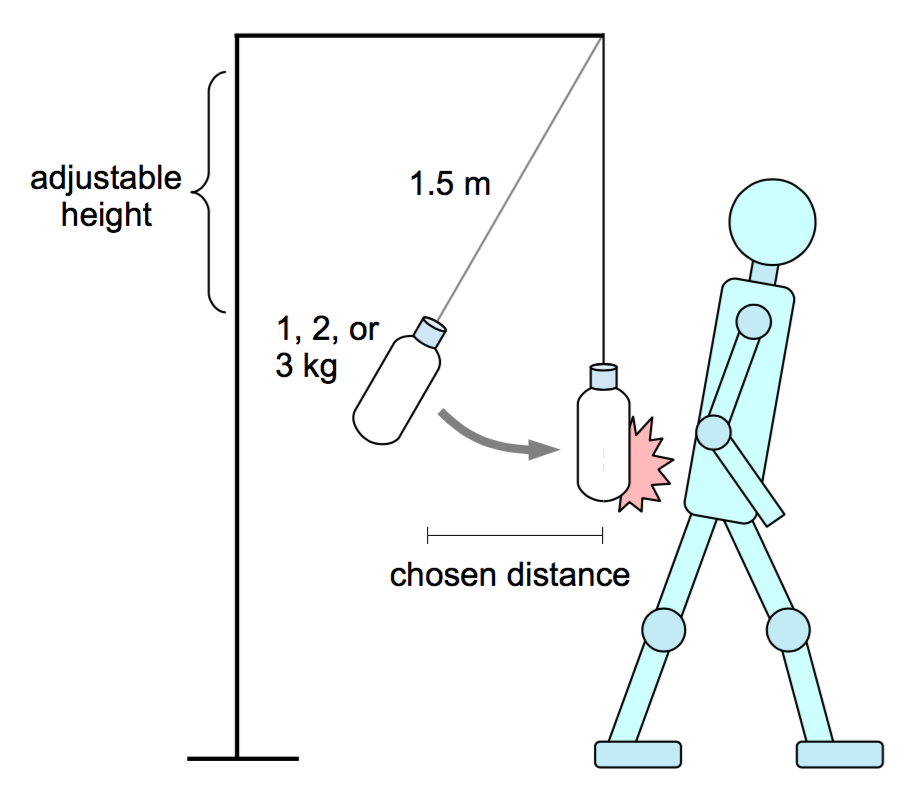
\includegraphics[height=6.5cm]{img/push_recovery.png}
\caption{Setup for the push recovery challenge. }
\end{center}
\end{figure}

\clearpage
\sffamily
{\bfseries\color[rgb]{0.4,0.4,0.4}
Part B: Goal-Kick from Moving Ball}
\phantomsection
\addcontentsline{toc}{subsection}{Part B: Goal-Kick from Moving Ball}


\bigskip

\added{The goal of the goal-kick from a moving ball challenge is to kick a moving ball
into the goal. Results of the technical challenge are based on a batch of three runs.}

\bigskip

\added{{\bfseries Run Setup}}

\smallskip

\begin{figure}[h]
\begin{center}
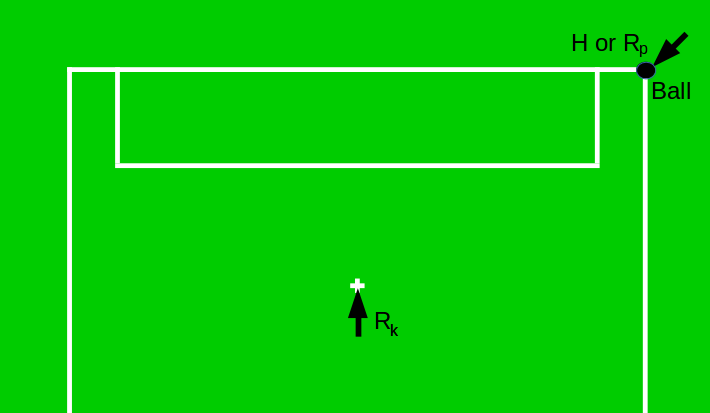
\includegraphics[width=0.6\textwidth]{img/tc_dynamic_kick.png}
\caption{\label{fig:tc_dynamic_kick}Setup for the moving ball challenge.}
\end{center}
\end{figure}

\added{The initial setup of a run is presented in Fig.~\ref{fig:tc_dynamic_kick},
procedure is as follows:}


\begin{enumerate}
\item \added{The ball is placed on one corner of the field as chosen by the team taking the
technical challenge.}
\item \added{The robot $R_K$ is placed on the penalty mark.}
\item \added{The pass of the ball may either be performed by a human member from the
team $H$ or another robot, $R_P$. If the pass is performed by a robot, the team
may place $R_P$ after the referee has placed the ball. $R_p$ can be placed
anywhere on the field, not directly touching the ball.}
\item \added{The referee blows the whistle to start the trial.}
\item \added{Teams may start the robot $R_P$ manually by pressing a button when the
trial starts. But $R_K$ must not be touched after the referee blew the whistle.}
\item \added{A chronometer is started when $R_P$ or $H$ kicks the ball.}
\end{enumerate}

\added{{\bfseries Run evaluation}}

\smallskip

\added{The chronometer is stopped when the trial ends. The causes for trial ends and
the possible results are as following:}
\begin{itemize}
\item \added{\textit{Failure}}
  \begin{itemize}
    \item \added{The ball has been touched twice by $R_P$, $H$ or $R_K$.}
    \item \added{$R_k$ attempted to kick but failed to touch the ball.}
    \item \added{The ball was kicked by $R_k$ but leaves the field without scoring a goal.}
  \end{itemize}
\item \added{\textit{Retake}}
  \begin{itemize}
    \item \added{The ball stops before $R_k$ attempted to kick.}
    \item \added{The ball \emph{bounced} on $R_k$ rather than being kicked.}
  \end{itemize}
\item \added{\textit{Partial success}}
  \begin{itemize}
    \item \added{Ball was kicked by $R_k$ but stopped rolling inside of the field.}
  \end{itemize}
\item \added{\textit{Success}}
  \begin{itemize}
    \item \added{Ball was kicked by $R_k$ and a goal was scored.}
  \end{itemize}
\end{itemize}

\added{{\bfseries Trials and ranking}}

\added{A trial consists of three different runs, each run ending with a \textit{Retake}
is restarted and do not count. A trial is considered as successful if at least 2
runs from the batch resulted in \textit{Success}. A trial is considered as
partially successful if at least 2 runs resulted in \textit{Success} or \textit{Partial success}.}

\added{The teams are ranked according to the following criteria on their best batch:}
\begin{enumerate}
\item \added{Number of \textit{Success} where the pass of the ball was executed by a robot}
\item \added{Number of \textit{Success} where the pass of the ball was executed by a human}
\item \added{Number of \textit{Partial success} where the pass of the ball was executed by a robot}
\item \added{Number of \textit{Partial success} where the pass of the ball was executed by a human}
\item \added{Average time for \textit{Success} runs, from first touch by $R_p$ or $H$ until goal is scored}
\item \added{Average shortest distance to the goal line for \textit{Partial success} runs}
\end{enumerate}


\removed{
The referee places the ball randomly on one corner of the goal area located on
the goal line. The robot $R_K$ is placed on the penalty mark. The pass of the
ball may either be performed by a human member from the team $H$ or another
robot, $R_P$. If the pass is performed by a robot, the team may place $R_P$
after the referee has placed the ball anywhere on the field not directly
touching the ball. The referee blows the whistle to start the trial. Teams may
start the robot $R_P$ manually by pressing a button when the trial starts.  }

\removed{
After the ball has been kicked by $R_P$ or the human, $R_K$ must
make contact with it before the ball comes to a stop, otherwise the trial is
unsuccessful. The trial is also unsuccessful if the ball leaves the field, $R_K$
touched the ball without the ball moving, or after one minute has elapsed since
the start of the trial. If after the ball contact the ball enters the goal, the
trial is successful and the time is stopped at the moment the ball passed the
goal line. Otherwise the trial is partially successful. Teams are first ranked
by the time for fully successful trials and then by the shortest distance
between the ball and the goal for partially successful trials.
}

\clearpage
\sffamily
{\bfseries \color[rgb]{0.4,0.4,0.4} Part C: High Jump}
\phantomsection
\addcontentsline{toc}{subsection}{Part C: High Jump}


\bigskip

The goal of the high jump challenge is to terminate ground contact and to stay in the air as long as possible. Robots are placed on a contact device \removed{of approximately 40 {\texttimes} 40 cm that records the time of flight of a jump} \added{or clearly marked area of approximately 60 {\texttimes} 60 cm}. A fully successful jump requires the robot to remain upright for a minimum of 3 seconds after landing without leaving the measuring device \added{or clearly marked area}. All other attempts are considered partially successful. \added{This includes attempts in which the robot handler touched the robot after landing but before the 3 seconds have exceeded.} The robots are ranked first according to the time of flight of fully successful attempts and then according to the time of flight of partially successful attempts.
\clearpage
\sffamily
{\bfseries\color[rgb]{0.4,0.4,0.4} Part D: High-Kick Challenge}
\phantomsection
\addcontentsline{toc}{subsection}{Part D: High-Kick Challenge}


\bigskip

The goal of the high-kick challenge is to kick the ball in the goal at maximum height. At each attempt, the team announces the minimum height their robot tries to achieve. The minimum height must be at least \removed{1/3rd} \added{2/3rd} of the ball's diameter and must be a multiple of 1cm.

The ball is then placed on the penalty mark and the team may position the robot freely but at least 30cm away from the ball. After the start signal, the robot may move the ball to any position before attempting a kick from the ground. Only kicks count that score a goal of at least the minimum height. The trial ends unsuccessfully when the ball leaves the field, or when the robot touches the goal obstacle \added{or the ball touches the front of the goal obstacle}.

The robots are ranked by the maximum height they successfully managed to kick the ball into the goal.


\end{document}
